\section{Summary of Layers}
\label{sec:layers}
This section describes the types of geospatial features visualized in the Geo-FTADS tool, and how each type of feature is visualized. The available geospatial layers are then introduced, along with their data sources. For layers that synthesize multiple datasets, or whose derivation otherwise involves detailed methodology, the reader is directed either to later sections or separate publications that detail the methodology involved. Table \ref{tab:layers_summary} summarizes the available layers, along with the type of geospatial feature used to visualize each.

\begin{table}[H]
\centering
\begin{tabular}{P{8cm}P{5cm}} % Adjust the column widths as needed
\toprule % Thicker top line
\textbf{Data Layer} & \textbf{Geospatial Feature Type} \\ \midrule % Midrule for under header
Freight flows (highway) & Highway \\
\midrule % Thin line between rows
Freight flows (regional) & Area \\
\midrule % Thin line between rows
Well-To-Wheel emissions associated with regional flows & Area \\
\midrule % Thin line between rows
Funded infrastructure projects & Area and Highway \\
\midrule % Thin line between rows
Charging and alternative fueling stations & Point \\
\midrule % Thin line between rows
Hydrogen production facilities & Point \\
\midrule % Thin line between rows
Locations of truck stops and principal ports & Point \\
\midrule % Thin line between rows
Demand charges & Area \\
\midrule % Thin line between rows
Grid emission intensity & Area \\
\midrule % Thin line between rows
Total cost of electric and diesel truck ownership & Area \\
\midrule % Thin line between rows
Total lifetime emissions of electric truck ownership & Area \\
\midrule % Thin line between rows
State-level incentives and regulations & Area \\
\midrule % Thin line between rows
Electricity demand by fully electrified trucking fleet & Area \\
\midrule % Thin line between rows
Available power capacity of the electrical grid & Area \\
\midrule % Thin line between rows
Pooled demand for truck stop charging & Point \\
\bottomrule % Thicker bottom line
\end{tabular}
\caption{Summary of data layers available in the Geo-FTADS tool.}
\label{tab:layers_summary}
\end{table}

\subsection{Feature Types and Visualization Methods}

The tool visualizes the available data layers as geospatial features, which fall into one of the following categories: area, highway, and point features. Each feature can be visualized as a gradient with respect to an associated attribute. The mechanism for visualizing the gradient varies depending on the type of feature.

\subsubsection{Area Features}
\textit{Area features} represent sets of areal regions separated by boundaries, such as US states. Attributes that can be visualized with respect to area features include commercial electricity price (visualized by state) and grid emission intensity (visualized by state or by balancing authority). Attributes are visualized by coloring the area of each region using a gradient from white (smallest attribute value) to solid red (largest attribute value). 

Fig. \ref{fig:area_features} shows two sample area features, and the right-hand figure illustrates the use of a color gradient to visualize an area attribute. 

\begin{figure}[ht]
    \centering
    \begin{subfigure}[b]{0.49\textwidth}
        \centering
        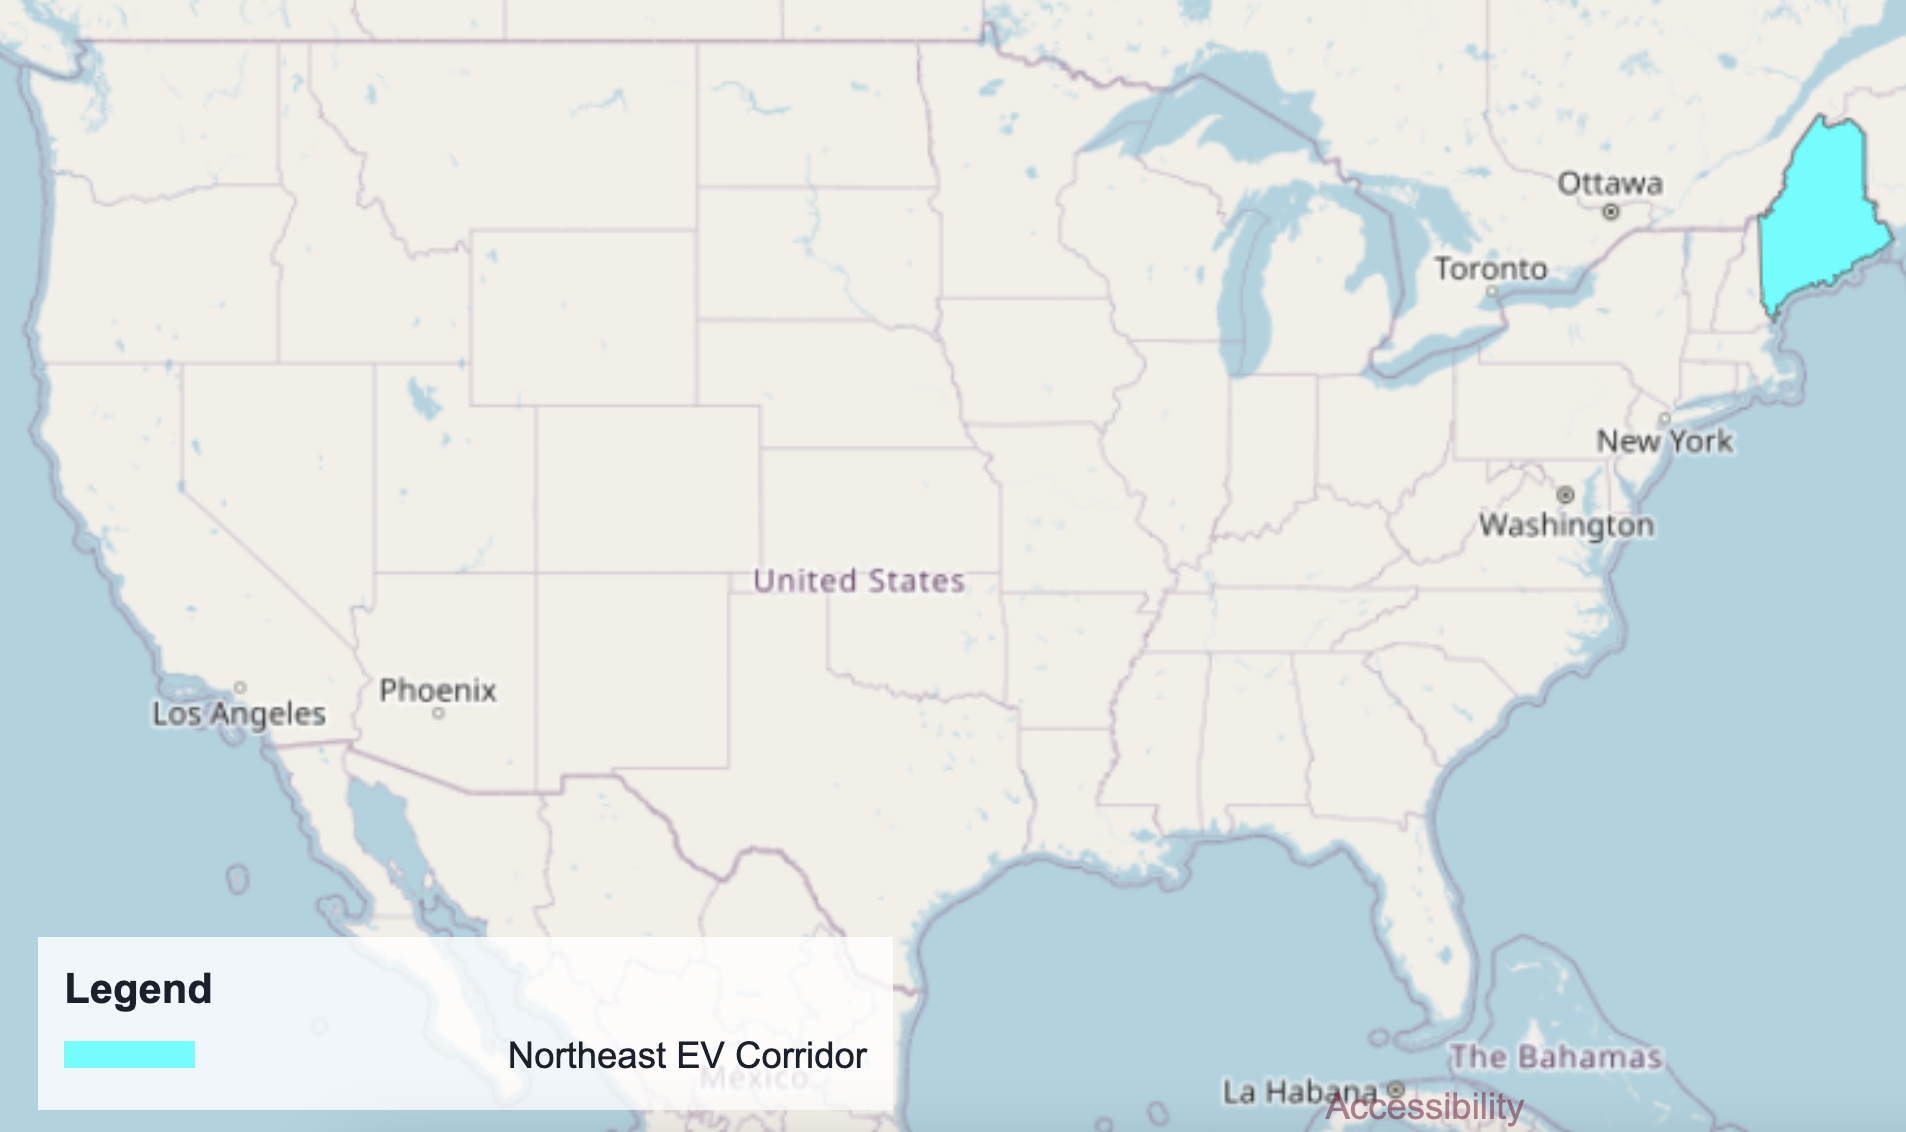
\includegraphics[width=\textwidth]{figures/northeast_ev_corridor.png}
        \caption{Northeast EV Corridor}
        \label{fig:northeast_ev_corridor}
    \end{subfigure}
    \hfill
    \begin{subfigure}[b]{0.49\textwidth}
        \centering
        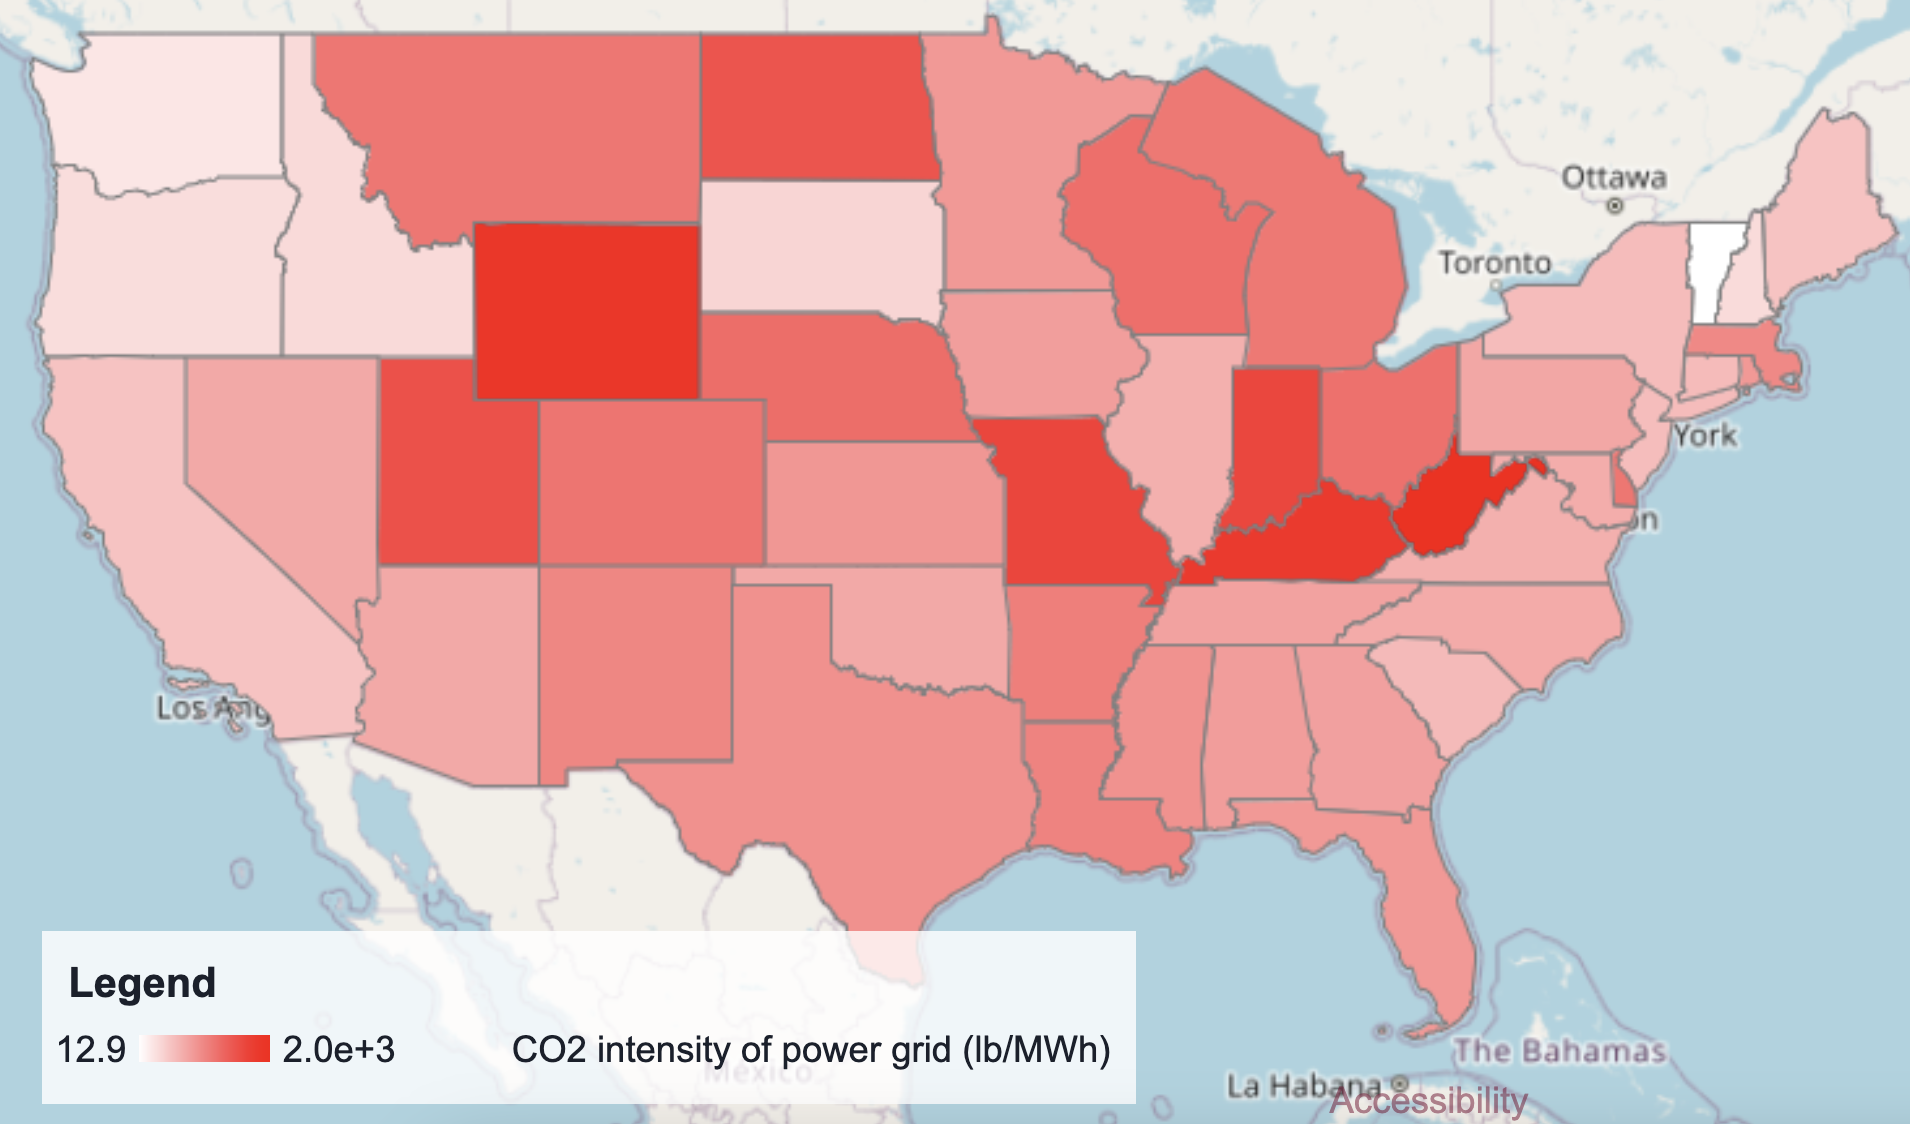
\includegraphics[width=\textwidth]{figures/grid_co2_intensity_state.png}
        \caption{Grid CO$_2$ intensity by US state.}
        \label{fig:grid_co2_intensity_state}
    \end{subfigure}
    \caption{Sample area features visualized with the geospatial mapping tool.}
    \label{fig:area_features}
\end{figure}

\subsubsection{Highway Features}

\textit{Highway features}, such as the U.S. interstate highway system, are represented by a network of connected straight lines. Each straight line in the network, referred to as a ``link", is typically less than one mile long, and connects end-to-end with other links to form the highway, as illustrated in Figure \ref{fig:highway_links_visual}.

\begin{figure}[ht]
    \centering
    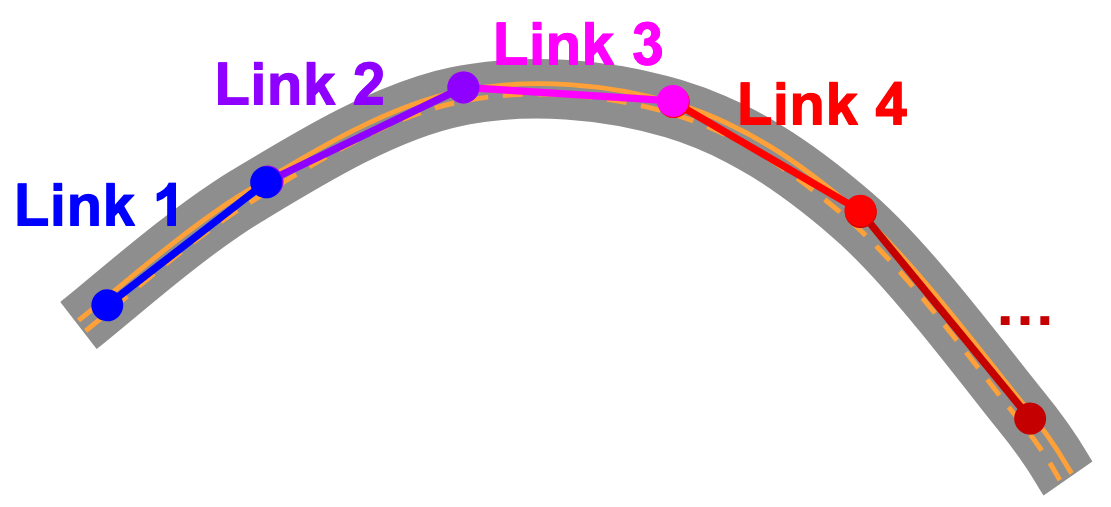
\includegraphics[width=0.5\textwidth]{figures/highway_links_visual.png}
    \caption{Illustration of highway links representing a curved section of highway.}
    \label{fig:highway_links_visual}
\end{figure}

Attributes such as the annual cargo mass carried over each link can be visualized by scaling the width of each link in proportion with the value of its associated attribute. Figure \ref{fig:highway_flows} illustrates the visualization of the U.S. interstate system with the Geo-FTADS tool. 

\begin{figure}[ht]
    \centering
    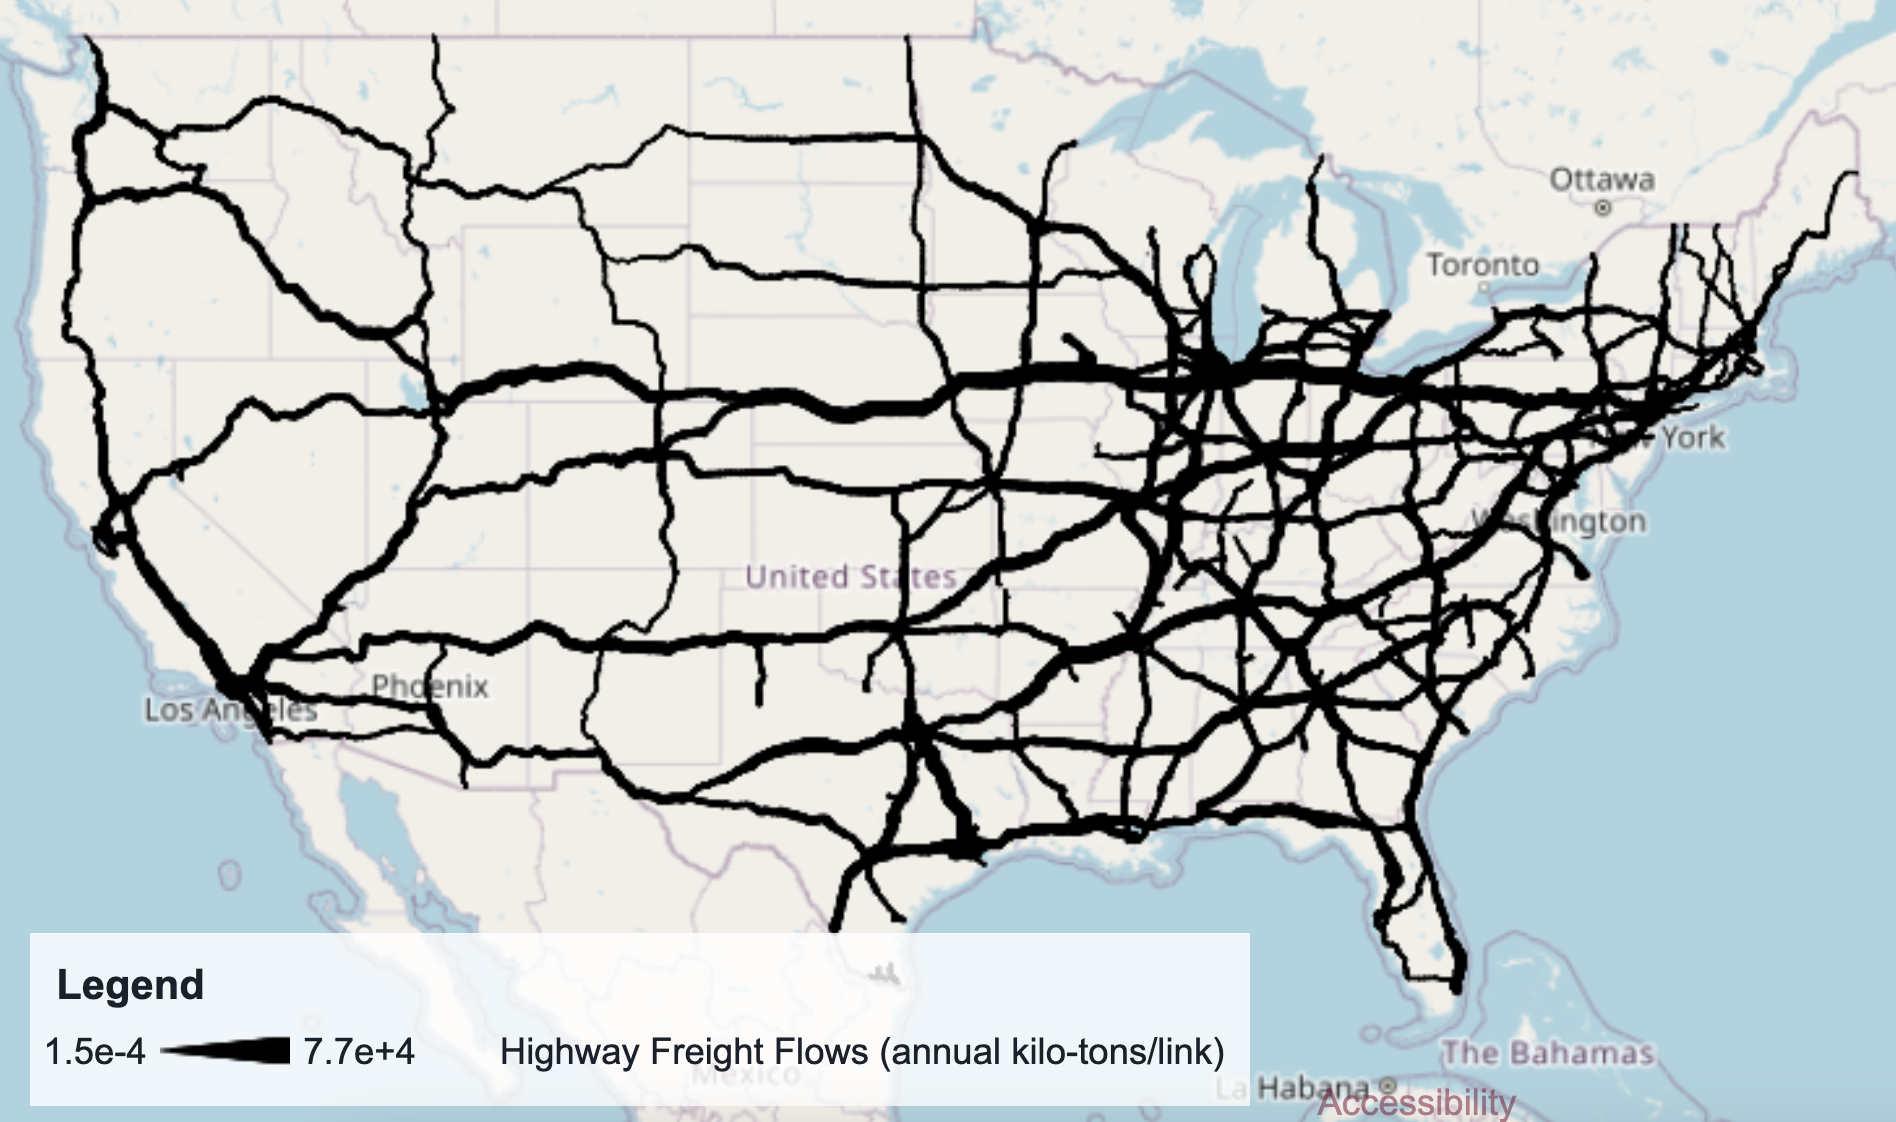
\includegraphics[width=0.7\textwidth]{figures/highway_flows.png}
    \caption{The U.S. interstate highway network, with a line width gradient used to visualize the annual cargo mass carried over each link.}
    \label{fig:highway_flows}
\end{figure}

\subsubsection{Point Features}

\textit{Point features} represent localized positions of objects on the map such as charging stations, truck stops and hydrogen production facilities. Point feature attributes, such as the installed power capacity of hydrogen production facilities, are visualized by weighting the diameter of each point in proportion with the value of its associated attribute. Figure \ref{fig:electrolyzer_facilities} illustrates the visualization of planned and operational electrolytic hydrogen production facilities with the tool. 

\begin{figure}[ht]
        \centering
        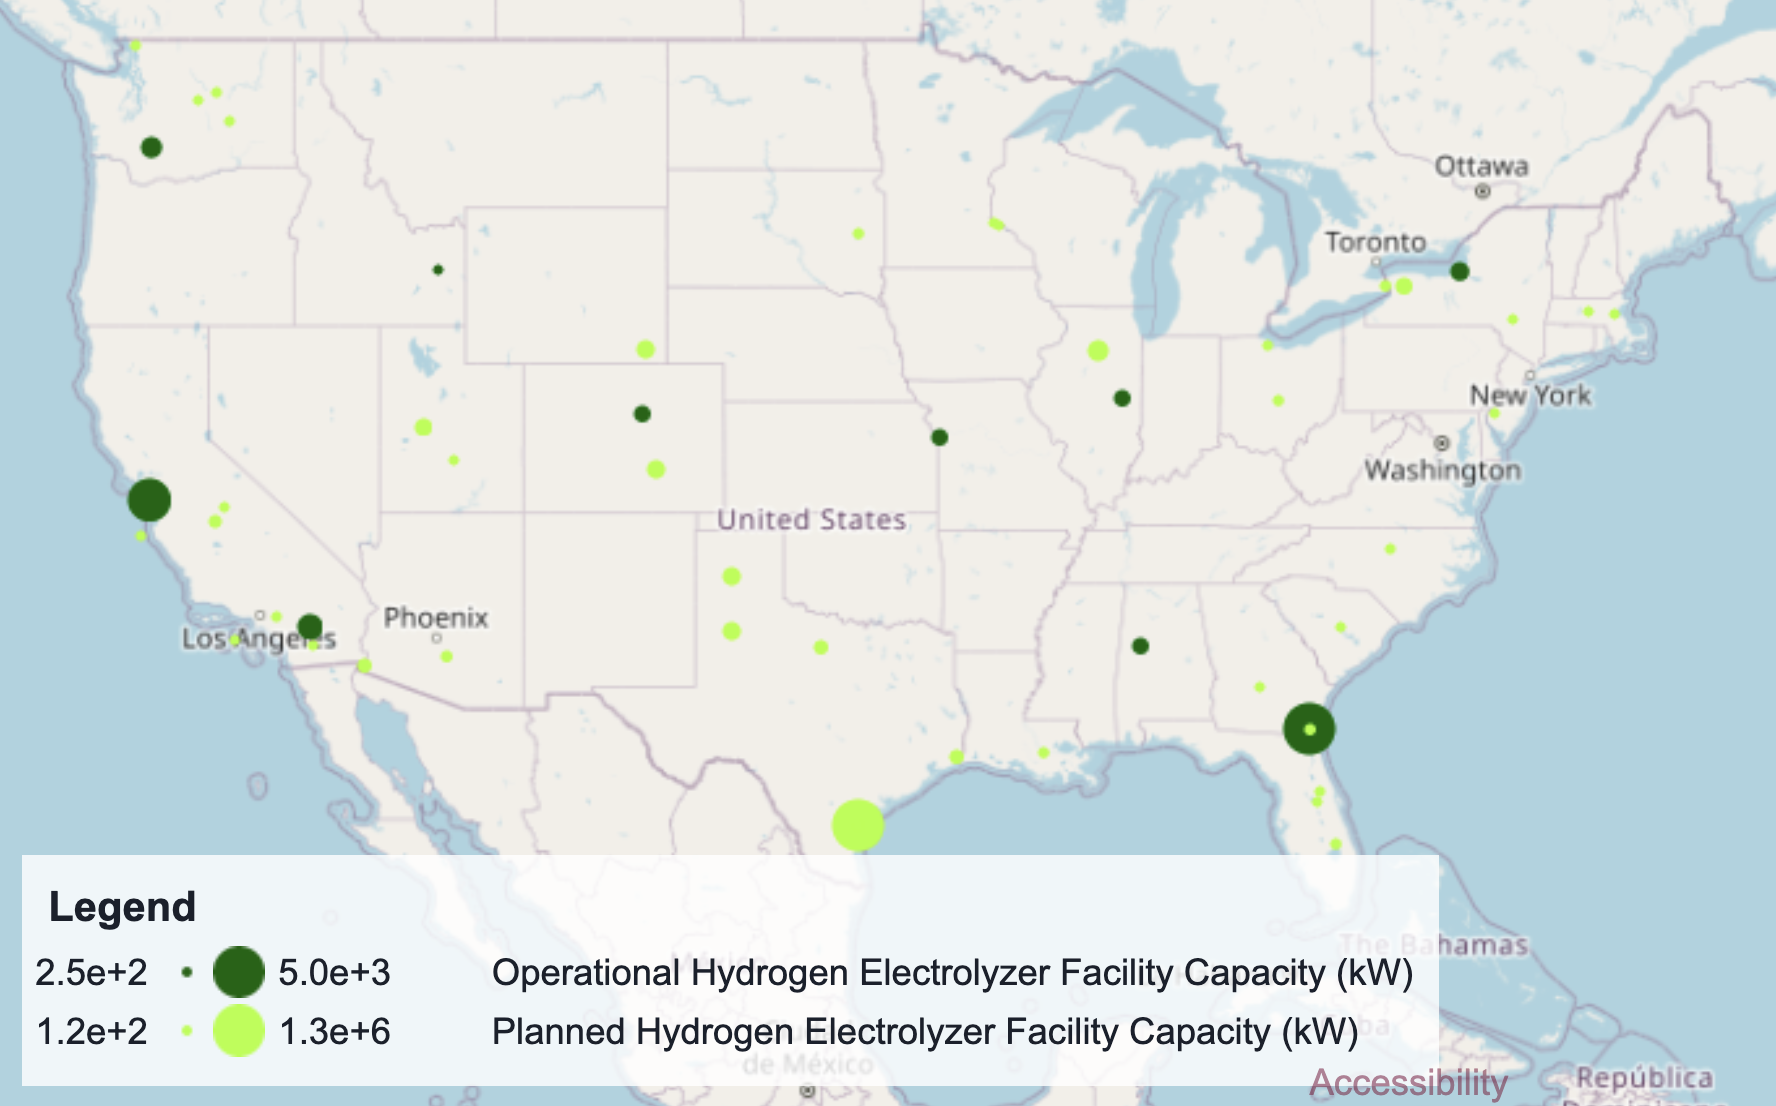
\includegraphics[width=0.7\textwidth]{figures/electrolyzer_facilities.png}
        \caption{Planned and operational electrolytic hydrogen production facilities in the U.S., with point diameter weighted by facility's power capacity.}
        \label{fig:electrolyzer_facilities}
\end{figure}

\subsection{Freight Flows}

To help target transition efforts to regions and corridors with high truck utilization, freight flows are visualized using data from the Freight Analysis Framework \cite{faf5_2024} maintained by the U.S. Department of Transportation. The freight flows can be visualized either between 132 regions of the US, referred to as ``FAF zones", or along highways. 

\subsubsection{Highway Flows}
Flows are visualized along each highway link using one of the following two link attributes: 1) annual flow of cargo carried over the link, or 2) the number of daily trips over the link. The annual flow of cargo carried over highway links in the U.S. interstate system is shown in Figure \ref{fig:highway_flows}.

\subsubsection{Regional Flows}
Flows between the FAF zones are available for a range of modes (truck, rail, pipeline, air), but the data visualized in the tool are filtered to only include freight carried by truck. The FAF5 data can be further filtered to visualize flows of specific commodities, broken down into 43 categories (cereal grains, wood products, etc.), and to visualize import and export flows separately. The ability to visualize flows of specific commodities can be especially helpful for companies that transport specialized goods, such as agricultural products. 

Regional flows are visualized as areal densities of cargo mass flow (ton-miles per square mile). The normalization by surface area (square miles) is done to eliminate any dependence on the sizes of origin and destination FAF5 zones. 

Figure \ref{fig:freight_flows} shows sample visualizations of regional freight flows densities. 

\begin{figure}[ht]
    \centering
    \begin{subfigure}[b]{0.49\textwidth}
        \centering
        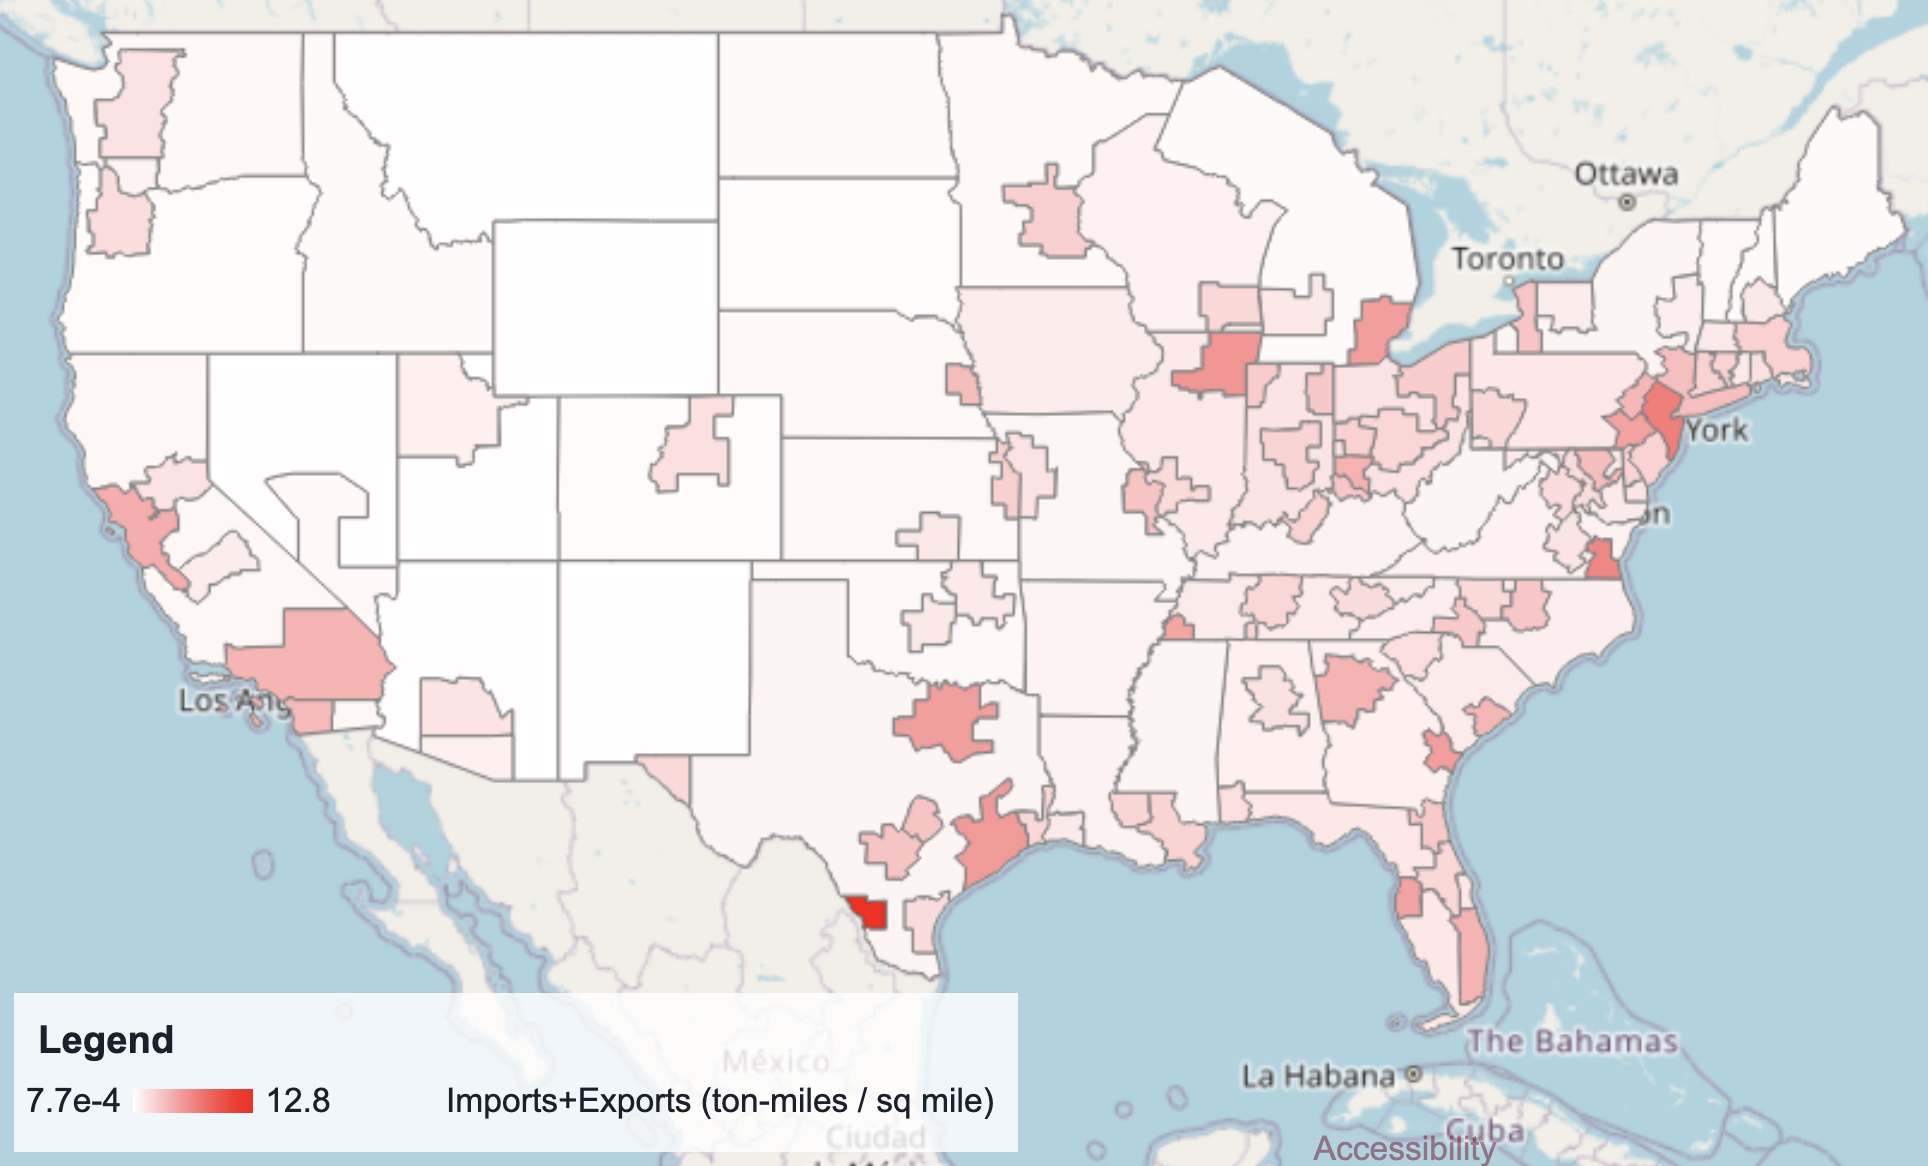
\includegraphics[width=\textwidth]{figures/imports_exports.png}
        \caption{Import and export flows (all commodities)}
        \label{fig:imports_exports}
    \end{subfigure}
    \hfill
    \begin{subfigure}[b]{0.49\textwidth}
        \centering
        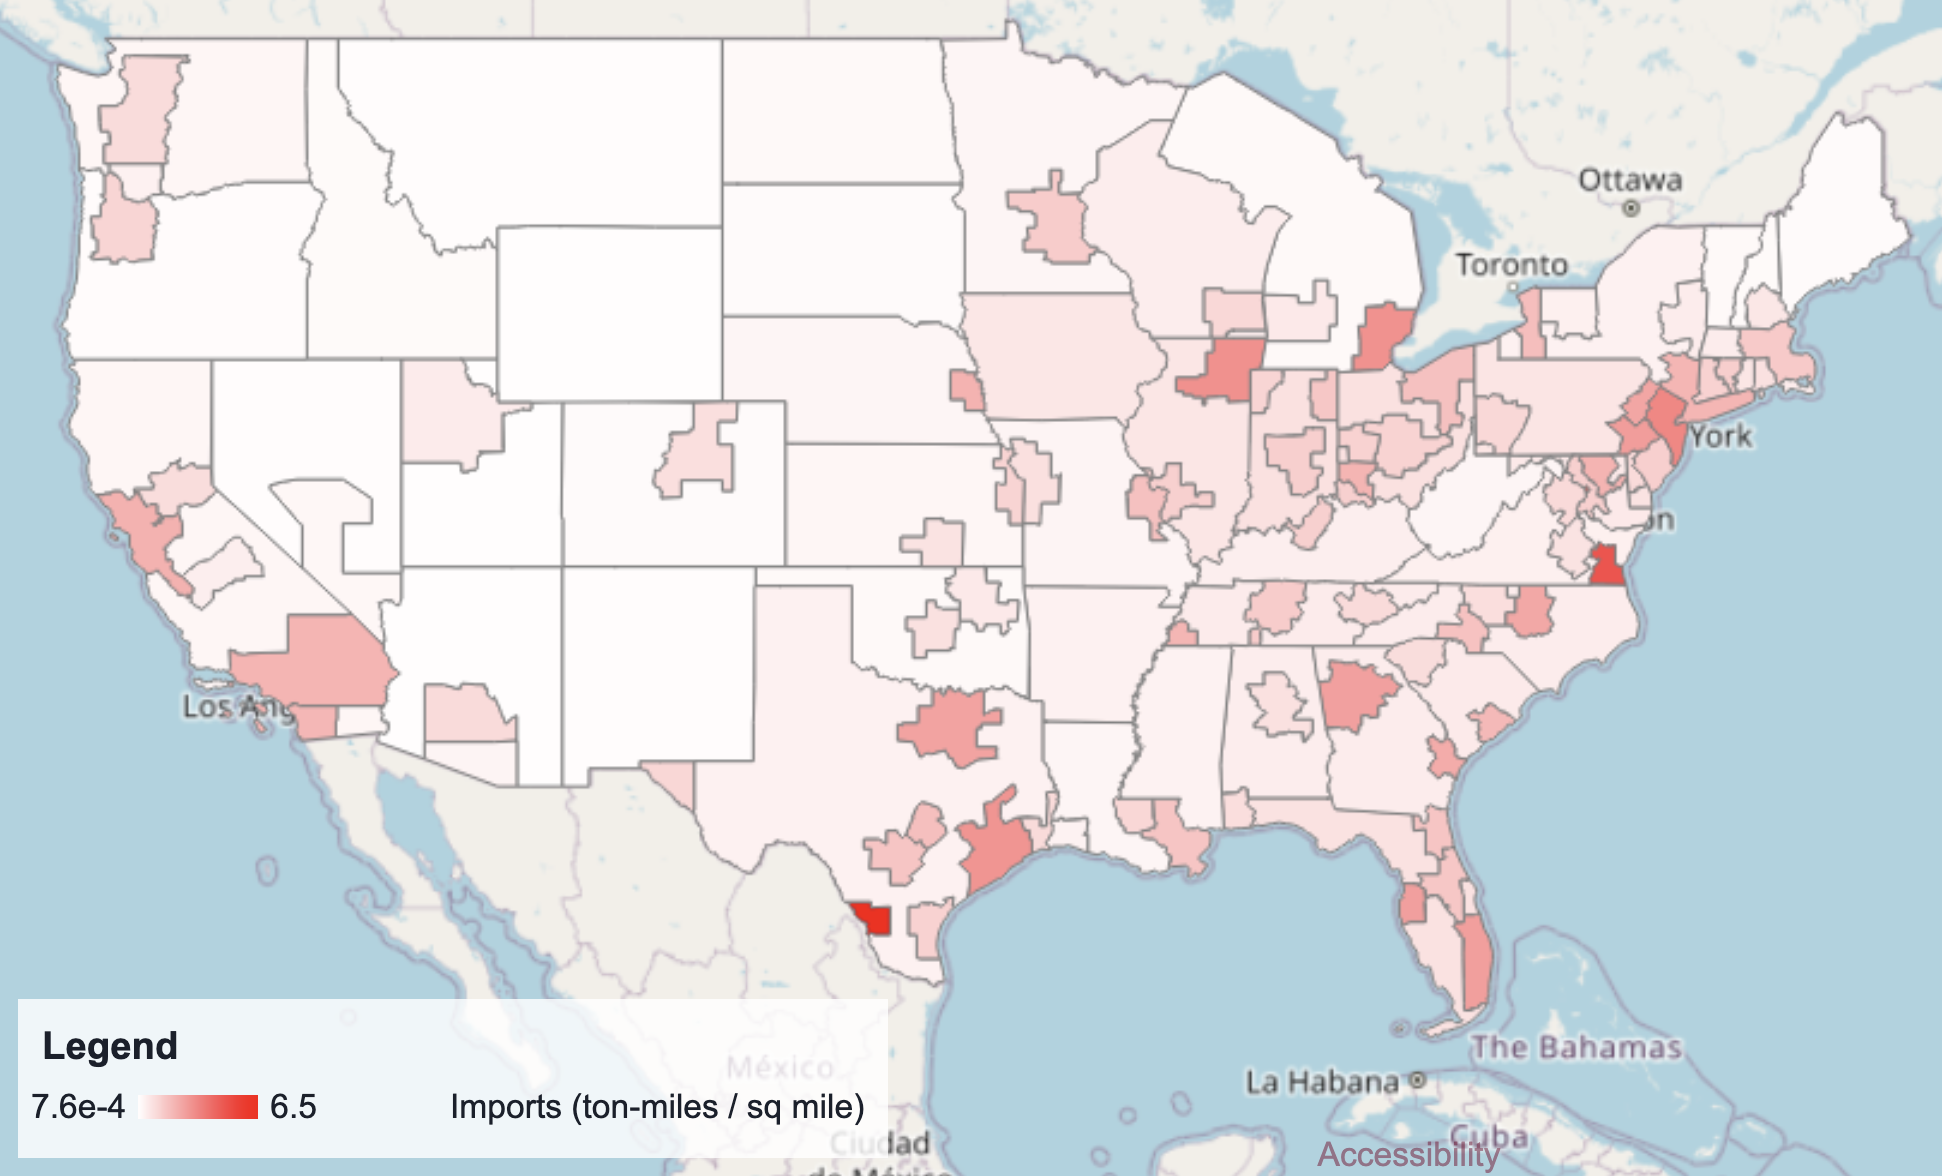
\includegraphics[width=\textwidth]{figures/imports.png}
        \caption{Import Flows (all commodities)}
        \label{fig:imports}
    \end{subfigure}
    \hfill
    \begin{subfigure}[b]{0.49\textwidth}
        \centering
        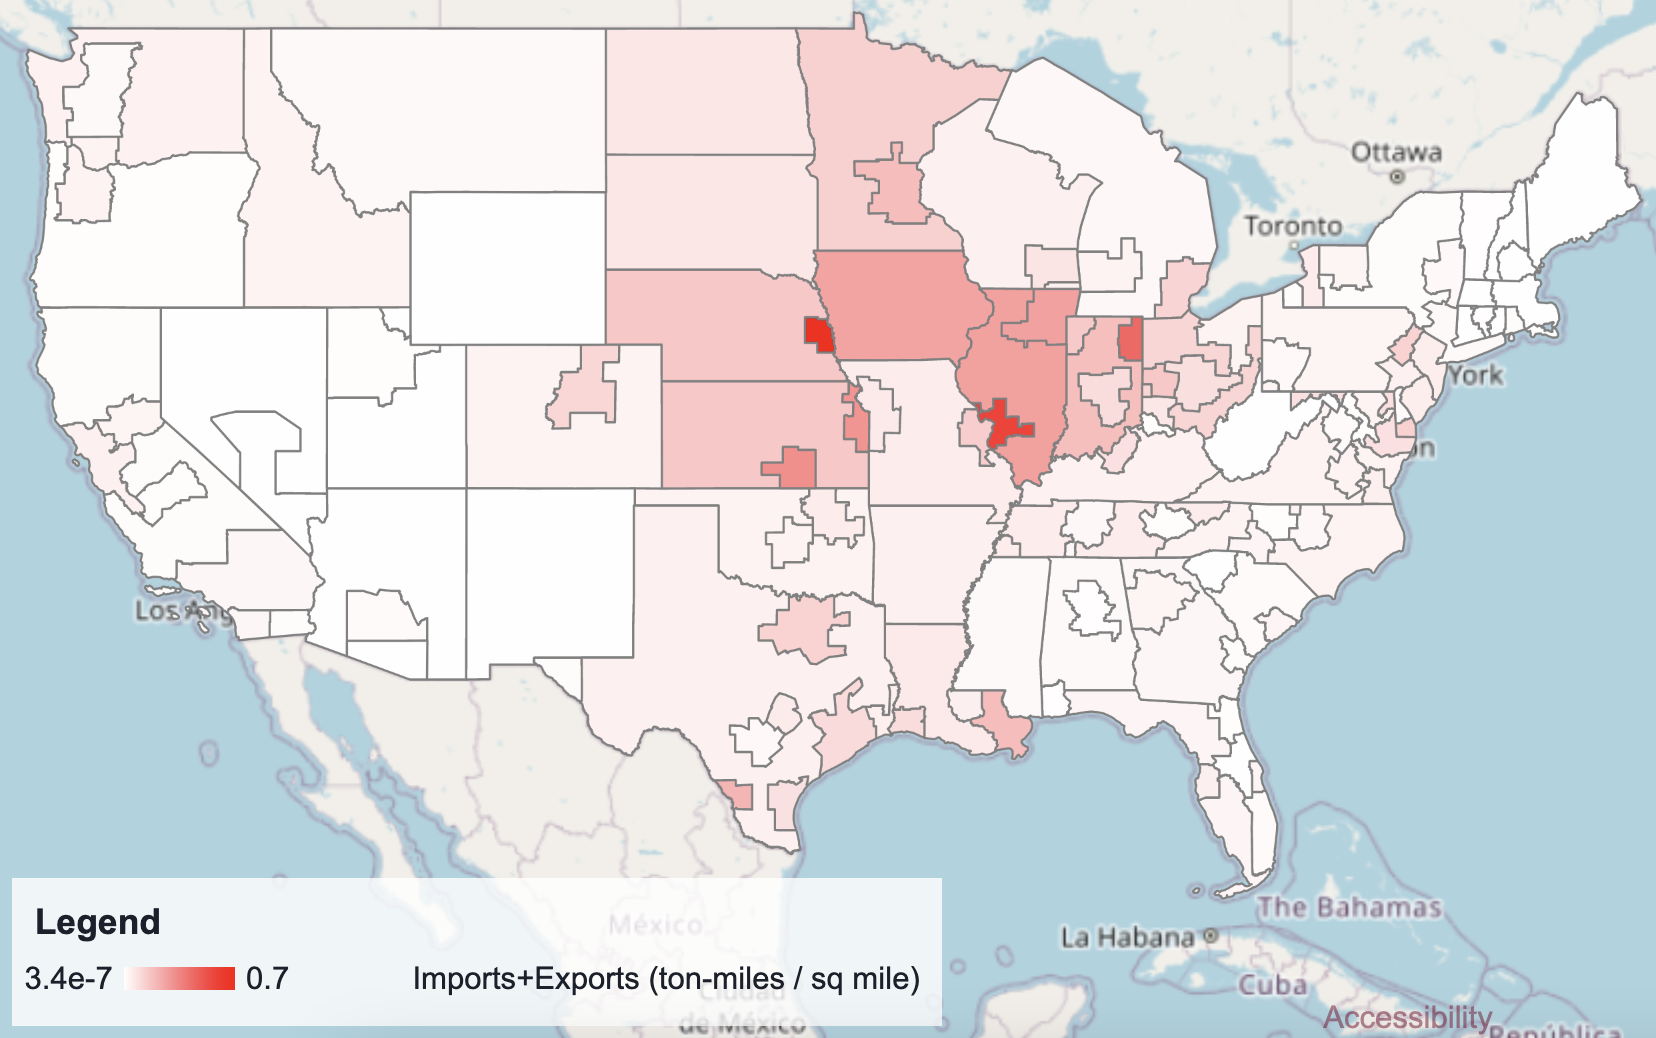
\includegraphics[width=\textwidth]{figures/imports_exports_cereal.png}
        \caption{Import and export flows (cereal grains)\newline}
        \label{fig:import_emissions}
    \end{subfigure}
    \caption{Sample visualizations of freight flow densities between FAF zones.}
    \label{fig:freight_flows}
\end{figure}

\subsection{Well-To-Wheel Emissions Associated with Regional Flows}

We have developed a methodology to combine the FAF5 data with fuel production and tailpipe emission intensities from the GREET model \cite{GREET_2022}, along with truck characteristics and operating conditions from the 2002 Vehicle Inventory and Use Survey \cite{VIUS_2002}, to evaluate approximate well-to-wheel emissions associated with interregional freight flows. Figure \ref{fig:import_export_emissions} shows the estimated well-to-wheel emissions associated with both import and export flows between the FAF zones for all commodities. 

\begin{figure}[ht]
    \centering
    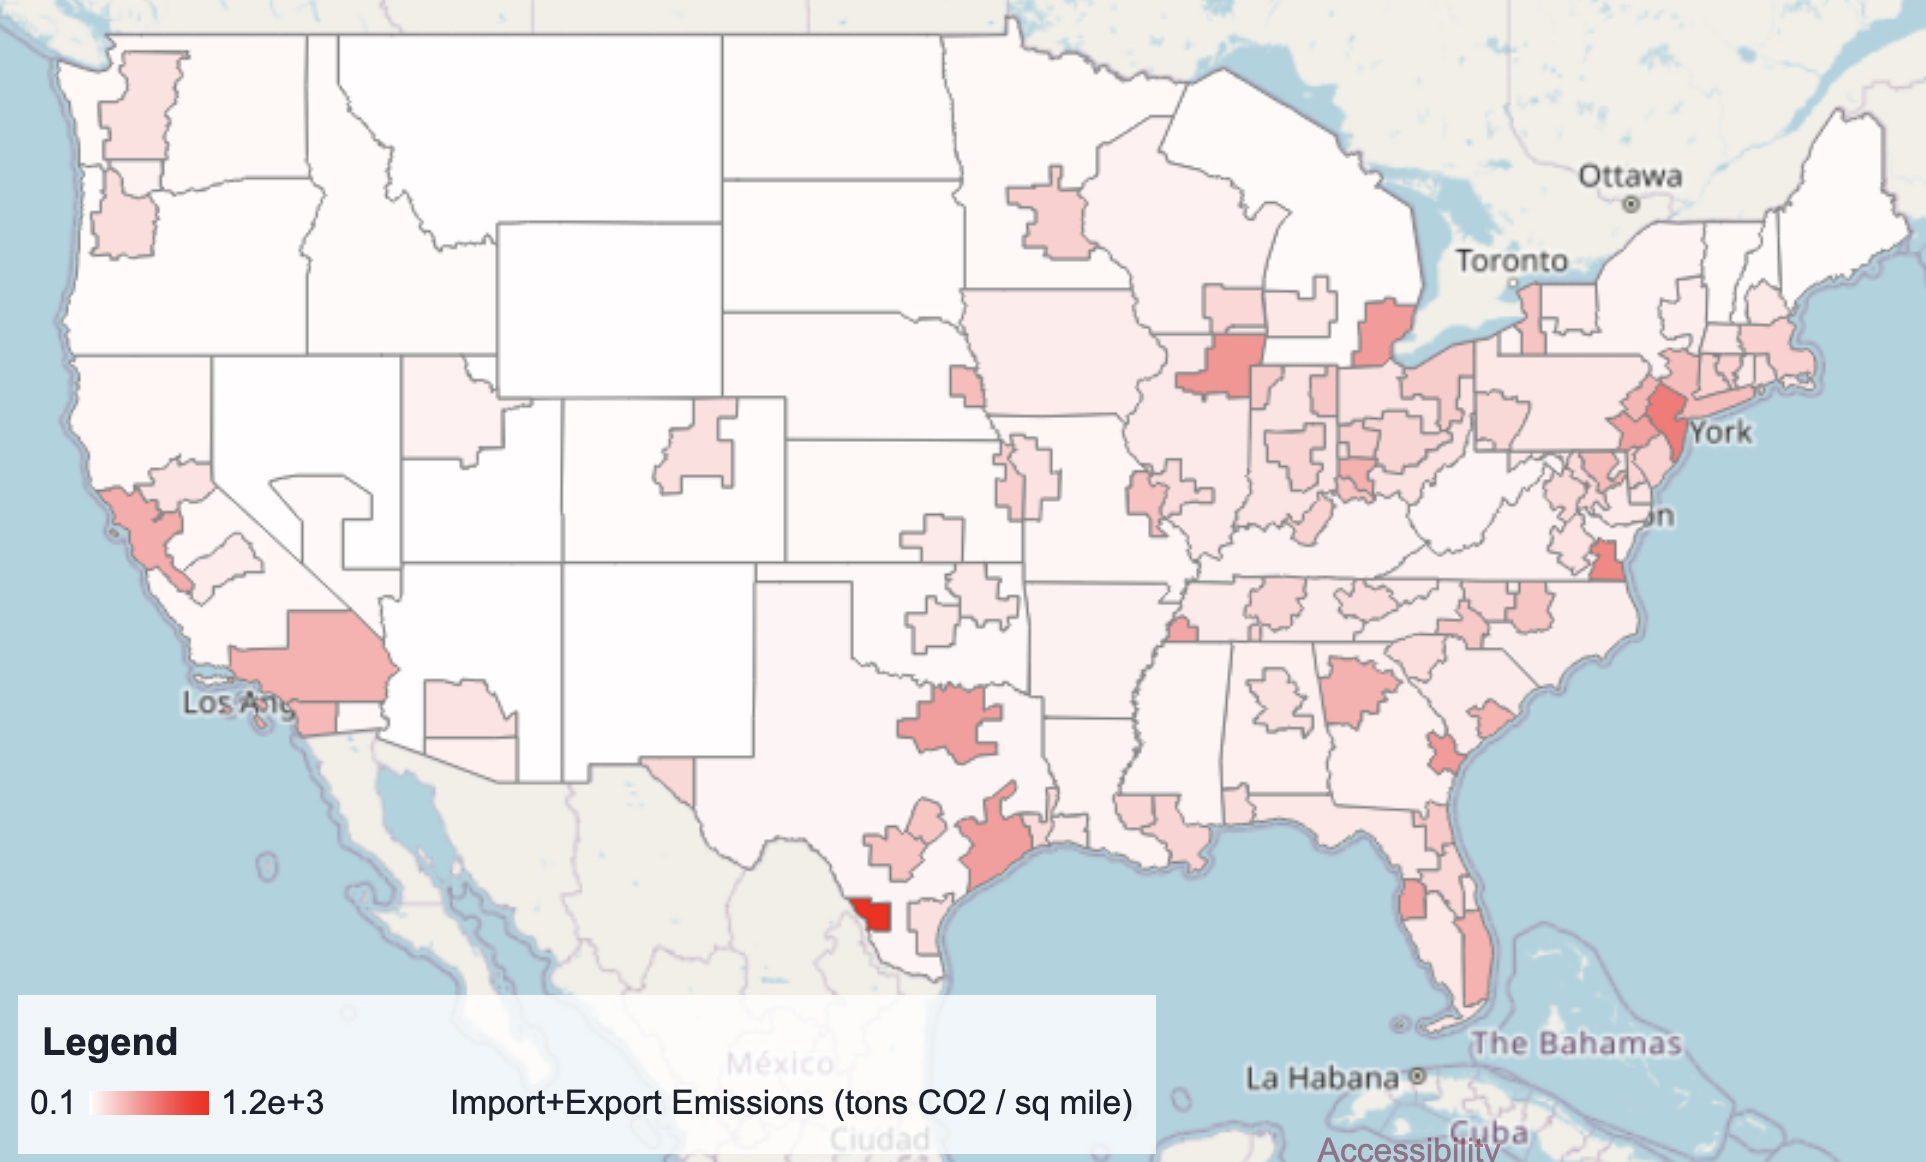
\includegraphics[width=0.7\textwidth]{figures/import_export_emissions.png}
    \caption{Well-to-wheel emissions associated with import and export flows (all commodities)}
    \label{fig:import_export_emissions}
\end{figure}

Under the current condition in which the vast majority (>99\%) of ton-miles are carried by diesel trucks, the emission rates are roughly proportional to the freight flows. Future work is needed to investigate how freight flow emissions changes with respect to penetration of alternative energy carriers, in which case we expect regional effects (eg. the regional intensity of the electrical grid) to become more pronounced. 

Section \ref{sec:freight_flows} provides details on the methodology developed to visualize emissions associated with regional freight flows. 

\subsection{Infrastructure}

The Geo-FTADS tool includes a variety of layers to visualize the locations and details of existing and planned infrastructure to support trucking fleets in transitioning to alternative energy carriers. 

\subsubsection{Funded Infrastructure Projects}

Layers to visualize the locations of seven zero-emission medium- and heavy-duty vehicle infrastructure projects funded by the US DOE and DOT are included to support stakeholders in coordinating fleet transition planning with anticipated locations of public infrastructure. The funding was announced by the Biden-Harris administration in 2023 to support the construction of zero-emission corridors and expansion of EV charging to underserved communities \cite{biden_harris_2023}. While some corridors, such as the Northeast EV Corridor \cite{NationalGridEVHighway} or the Houston to LA H$_2$ corridor \cite{H2LAAACOG2024}, target specific ZEV options, others such as the East Coast ZEV corridor \cite{CalstartZEVCorridor} aim to support both electric and hydrogen truck infrastructure. 

Figure \ref{fig:infra_projects} shows the four funded corridors, along with a sample region being targeted for EV charging expansion. 

\begin{figure}[ht]
        \centering
        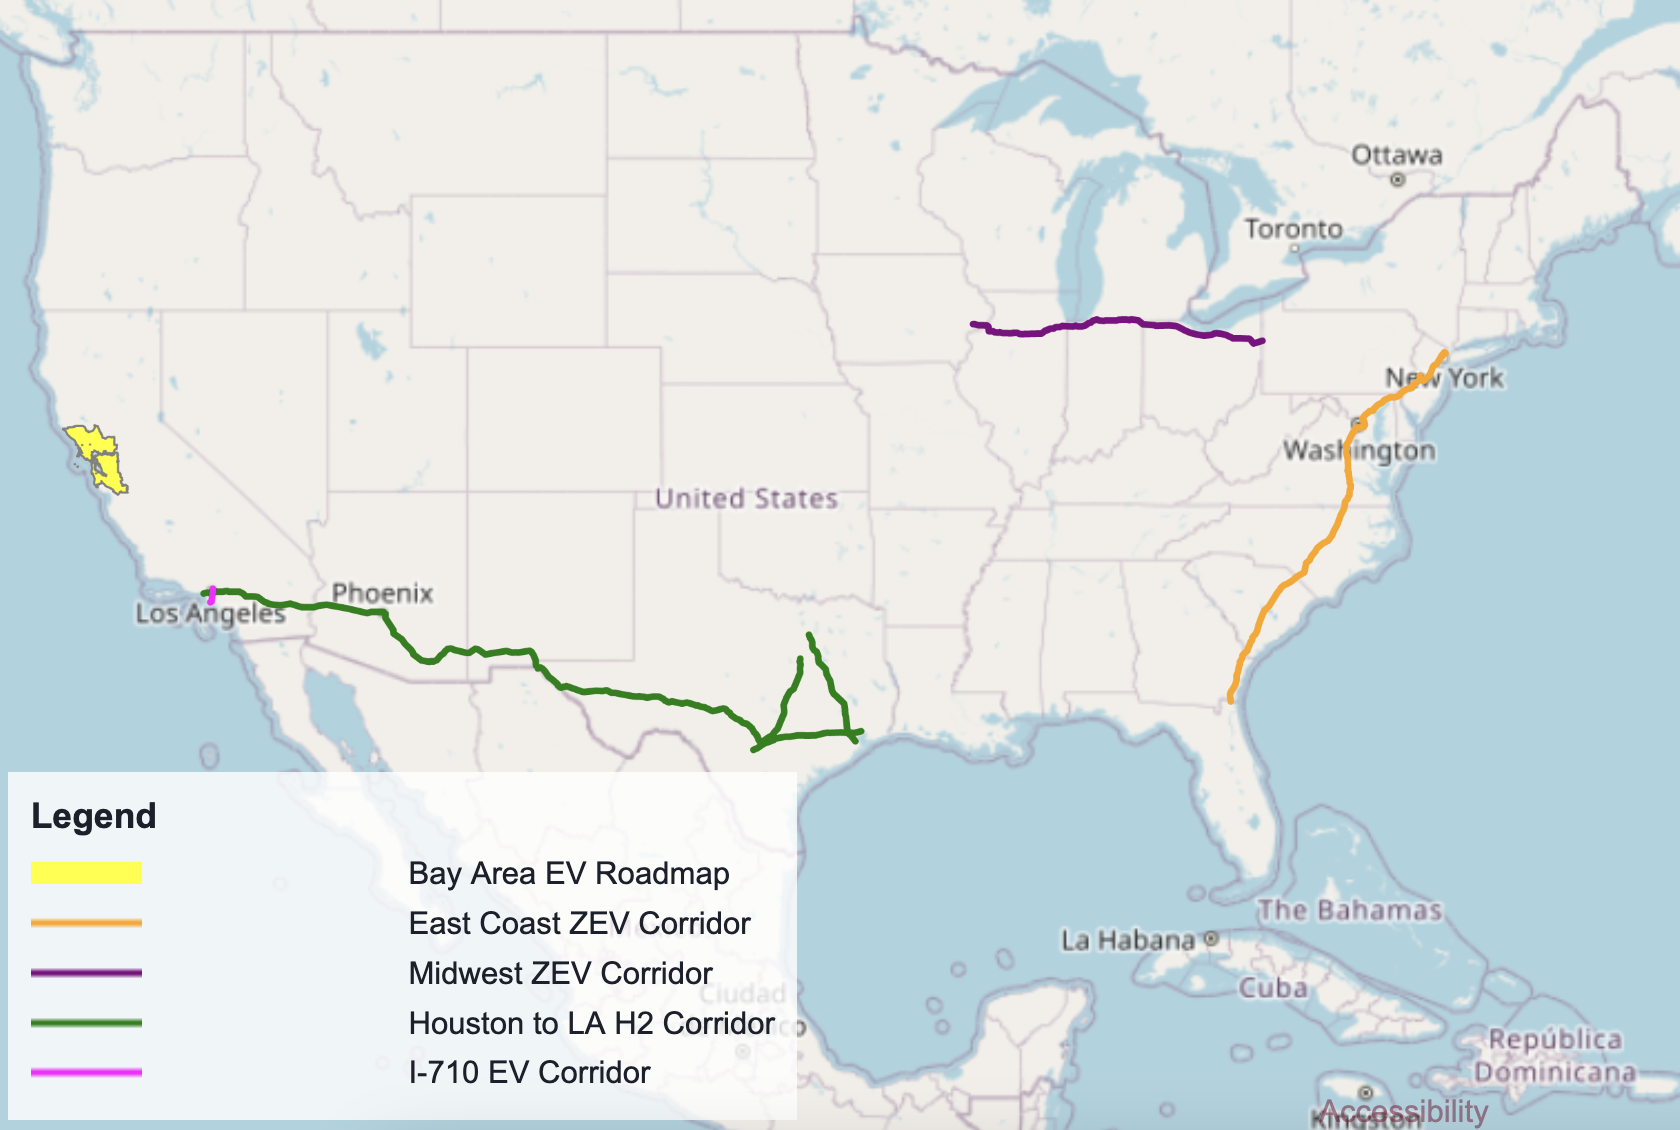
\includegraphics[width=0.7\textwidth]{figures/infra_projects.png}
        \caption{Corridors funded by the US DOE and DOT for zero-emission medium-and heavy-duty vehicle infrastructure, along with one of the three region (the Bay Area) targeted for expansion of EV charging infrastructure. }
        \label{fig:infra_projects}
\end{figure}

\subsubsection{Charging and Alternative Fueling Stations}

Current locations of public direct current fast charging (DCFC) and alternative fueling stations from the DOE Alternative Fuels Data Center \cite{AFDC_2024} can be visualized to support stakeholders in co-locating fleet transitions with supportive public infrastructure, as shown in Figure \ref{fig:stations}.

\begin{figure}[ht]
        \centering
        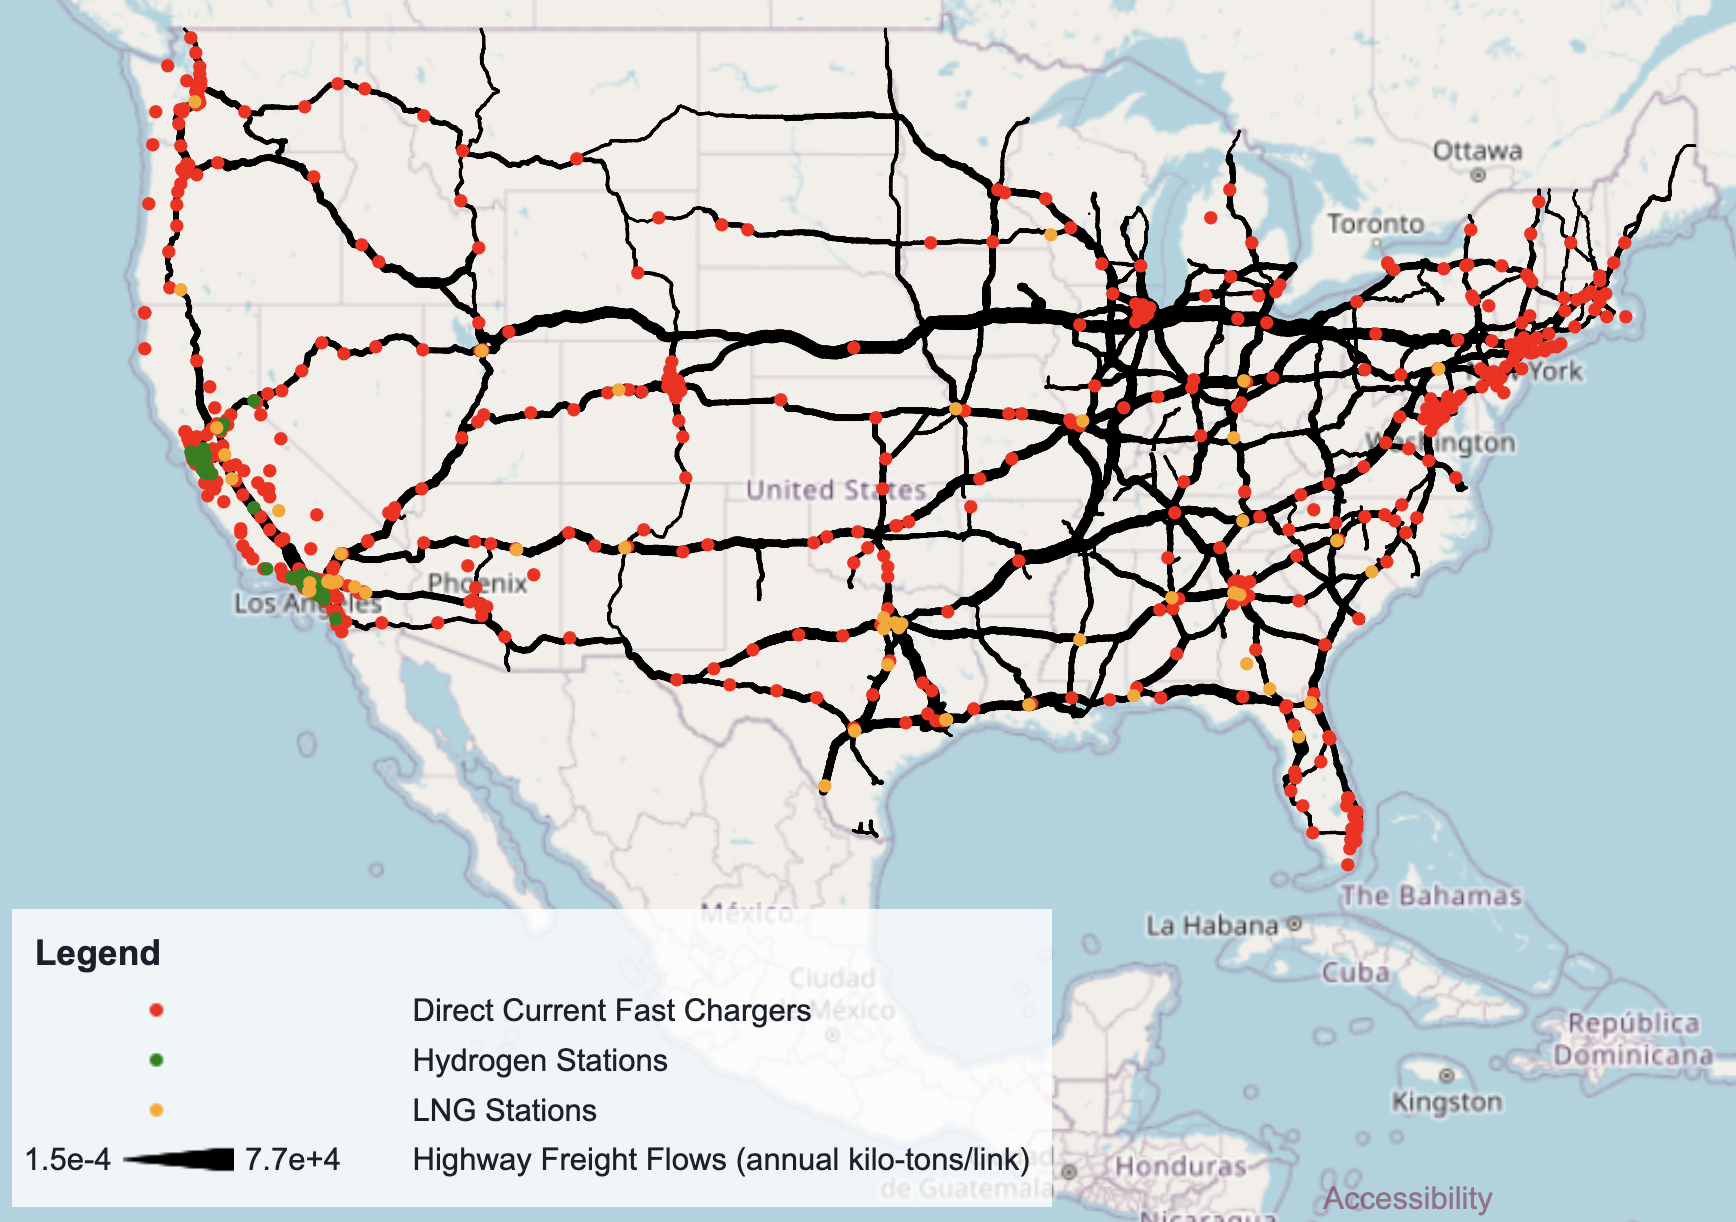
\includegraphics[width=0.7\textwidth]{figures/stations.png}
        \caption{Locations of DCFC and hydrogen and liquid natural gas (LNG) refueling stations, overlaid on the interstate highway network. Compressed natural gas (CNG) and liquid propane gas (LPG) stations are also available in the tool.}
        \label{fig:stations}
\end{figure}

A limitation of this dataset is that it does not indicate the suitability of most stations for use by medium and heavy-duty vehicles. In particular, most DCFCs are likely only usable by light-duty vehicles. However, a high density of DCFCs in a given region may still provide a strong indication of regional support for installation of EV charging stations, and of local grid infrastructure and capacity to support high charging powers that will be needed for many trucking applications.  

\subsubsection{Existing and Planned Hydrogen Production Facilities}

Locations of hydrogen production facilities that are either planned, under construction, or operational can be visualized, along with their hydrogen production capacities, as point features to help assess current and anticipated regional availability of hydrogen to support deployment of hydrogen trucking fleets. Operational facilities include both electrolyzers and oil and chemical refineries that produce hydrogen as a by-product. However, for planned and under-construction facilities, data is only available for electrolyzers (not refinery production).

Data on locations and production capacities was obtained from a 2023 DOE Hydrogen Program Record \cite{Hydrogen2023ElectrolyzerInstallations} for electrolyzer facilities, and from two complementary datasets \cite{H2ToolsCaptiveHydrogenProduction,H2ToolsMerchantHydrogenCapacities} from the Hydrogen Tools Portal \cite{H2Tools} for hydrogen produced at refineries. These data layers are shown in Figure \ref{fig:hydrogen_facilities}.

\begin{figure}[ht]
        \centering
        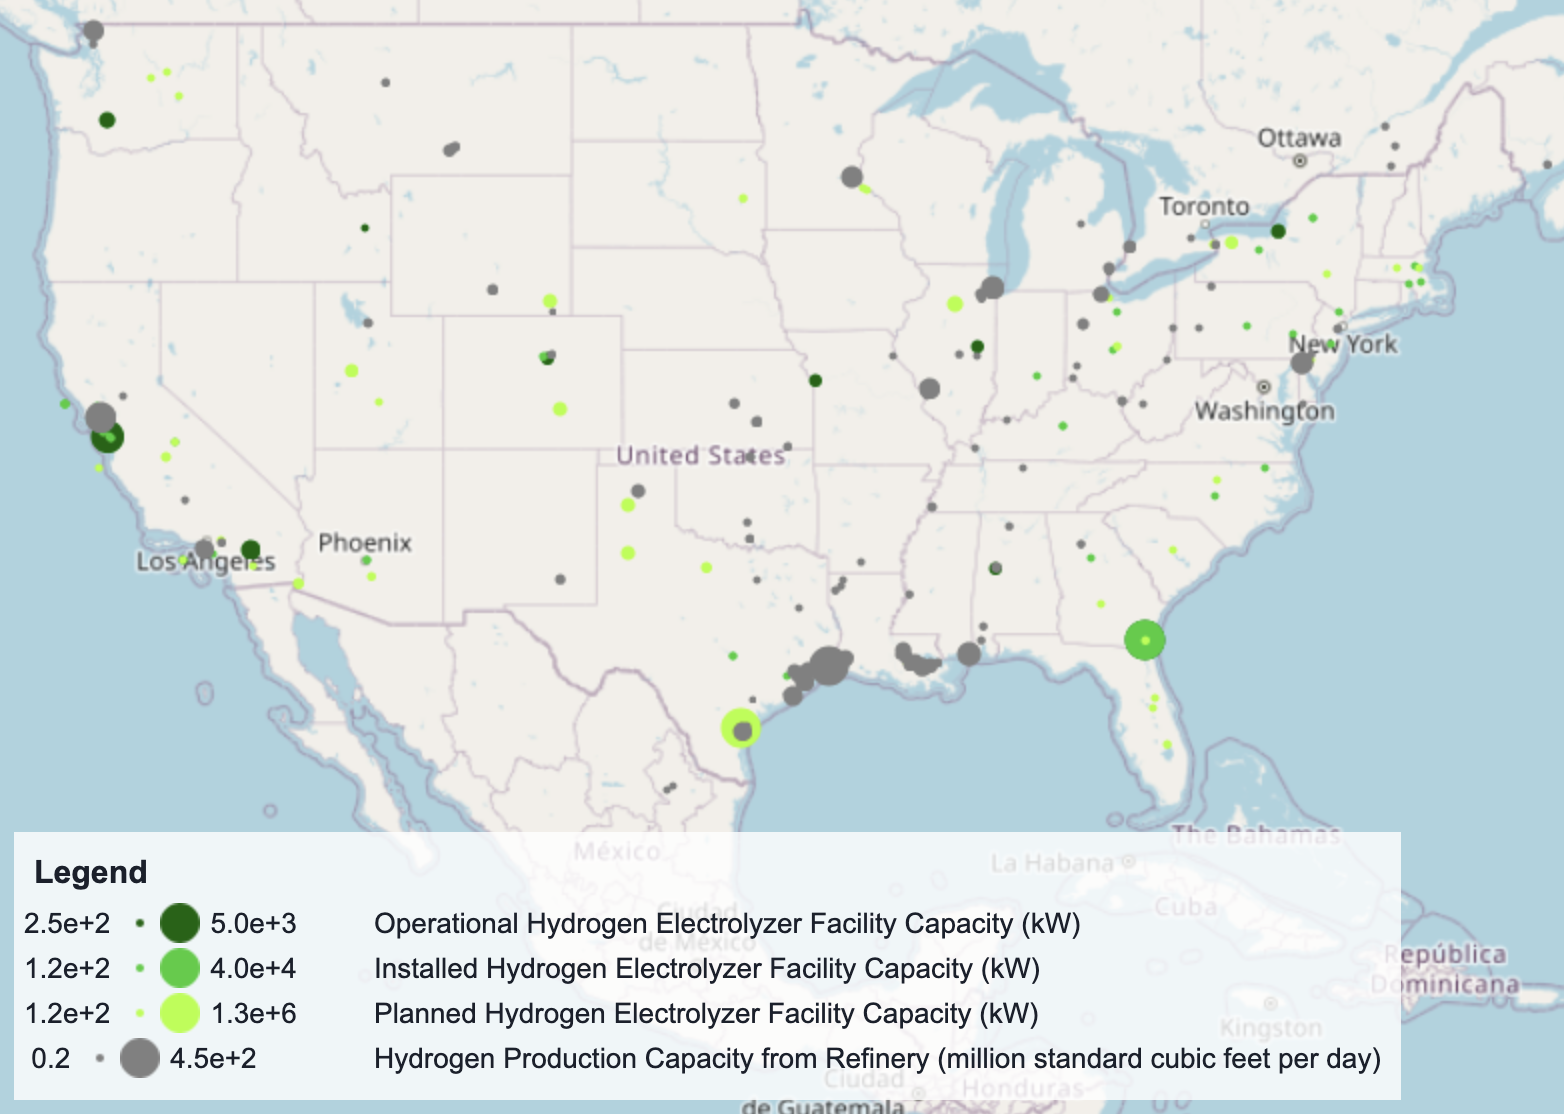
\includegraphics[width=0.7\textwidth]{figures/hydrogen_production_facilities.png}
        \caption{All hydrogen production facilities visualized on the geospatial mapping tool, along with their hydrogen production capacities.}
        \label{fig:hydrogen_facilities}
\end{figure}

\subsubsection{Locations of Truck Stops and Principal Ports}

Other point features available include the locations of truck stops and principal ports, which are intended to help infrastructure providers quickly locate potential hubs to target where vehicles already stop to refuel or load/unload cargo. 

\subsection{Costs and Emissions}

The tool includes several layers to support stakeholders in assessing transition costs and emissions. 

\subsubsection{Commercial Electricity Price, Demand Charges and Grid Emission Intensity}
\label{sec:elec_price_emissions_intensity}

The commercial electricity price from the EIA \cite{EIA_2024} and grid emission intensity from the eGRIDs database \cite{eGRID_2022} can be visualized for different US states to view fundamental regional inputs for cost and emissions assessments. 

Demand charges, which scale with a user's maximum instantaneous power demand over a given period \cite{FEMP_DemandCharge}, are especially relevant to trucking fleets due to the high powers (up to $\sim$1 MW \cite{Moorthy_2022}) that will be needed for $~$1h truck charging. Maximum utility demand charges at both the state and utility levels are evaluated using historical maximum demand charge data compiled by the National Renewable Energy Lab (NREL) \cite{McLaren_2017}. The maximum charge at the utility level is obtained by finding the maximum of all charges associated with a given utility ID in the historical dataset. At the state level, there are options to visualize either the maximum, mean or median of historical maximum demand charges over all utilities that overlap with the state. 

Figure \ref{fig:grid_costs} illustrates the demand charge and commercial electricity price layers. The grid emission intensity is shown in \ref{fig:grid_co2_intensity_state}.

\begin{figure}[ht]
    \centering
    \begin{subfigure}[b]{0.49\textwidth}
        \centering
        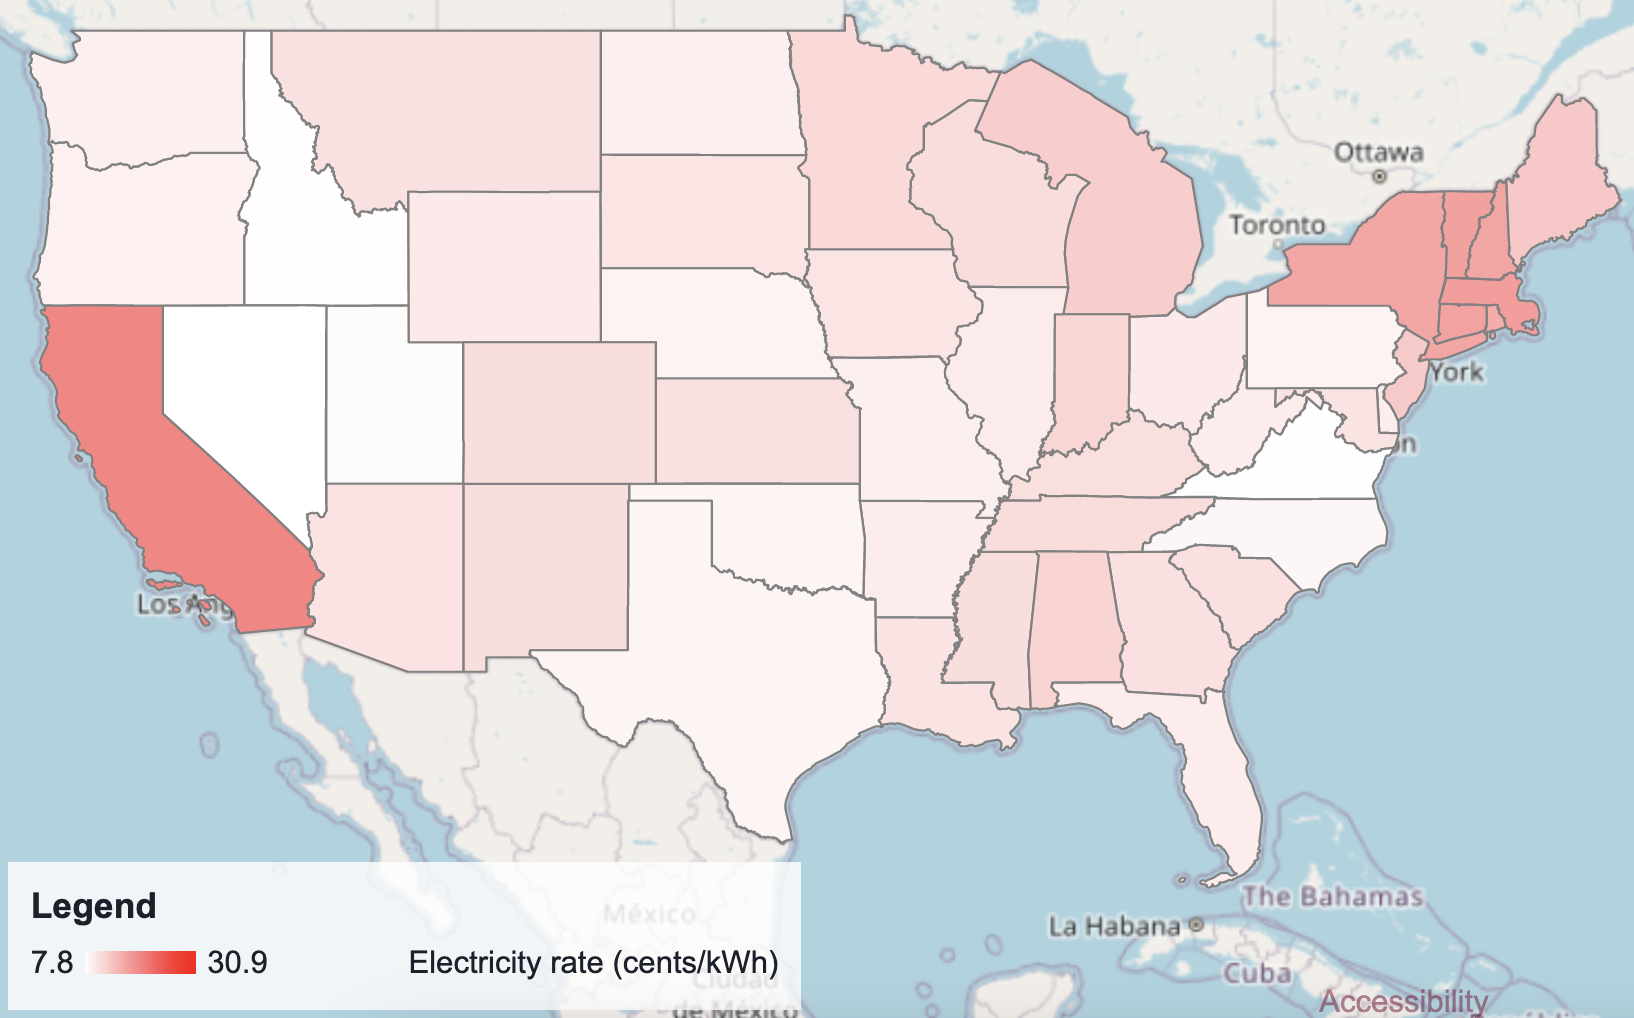
\includegraphics[width=\textwidth]{figures/commercial_electricity_price.png}
        \caption{Commercial electricity price}
        \label{fig:commercial_electricity_price}
    \end{subfigure}
    \hfill
    \begin{subfigure}[b]{0.49\textwidth}
        \centering
        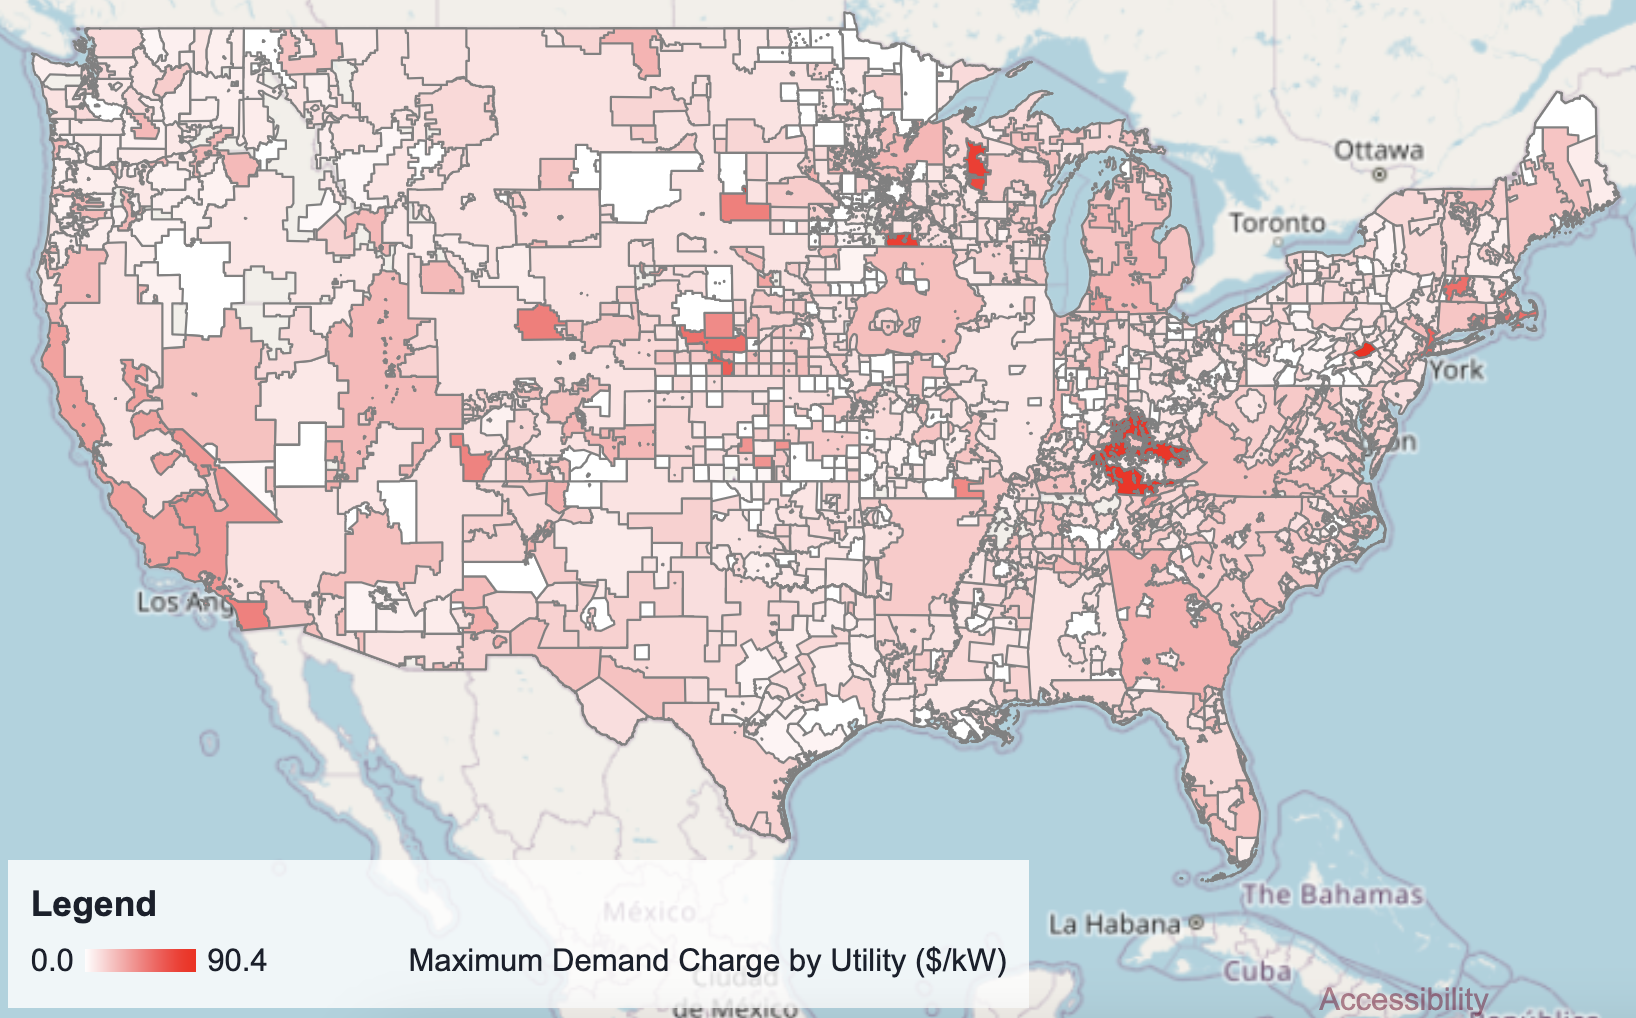
\includegraphics[width=\textwidth]{figures/demand_charge.png}
        \caption{Maximum utility-level demand charges}
        \label{fig:demand_charge}
    \end{subfigure}
    \caption{Fundamental regional layers used to evaluate fleet transition costs}
    \label{fig:grid_costs}
\end{figure}

\subsubsection{Total Costs and Emissions of Electric and Diesel Truck Ownership}

To support users in assessing cost and emission impacts of transitioning fleets to battery electric, layers are available for an adaptation of the EV truck model and analysis presented in \cite{Sader_2023}, which compares the total cost of ownership (TCO) and well-to-wheel emissions of EV vs. diesel long-haul trucking over a 10-year truck lifespan. To remain policy-agnostic, the total cost of ownership currently does not account for federal tax credits or state-level incentives available to support fleets in transitioning to battery electric.

The truck model presented in Ref. \cite{Sader_2023} is adapted to represent the Tesla Semi using data from PepsiCo's 2023 Tesla Semi pilot, which was undertaken in partnership with the Run on Less - Electric DEPOT demonstration \cite{NACFE_2023} launched by the North American Council for Freight Efficiency (NACFE) and the Rocky Mountain Institute (RMI). Flexibility has also been added to the model to represent a wider range of operating profiles. 

Figure \ref{fig:truck_costs_emissions} shows a sample of these layers, and the methodology and assumptions used to adapt the model as described are discussed in more detail in Section \ref{sec:costs_emissions}.

\begin{figure}[ht]
    \centering
    \begin{subfigure}[b]{0.49\textwidth}
        \centering
        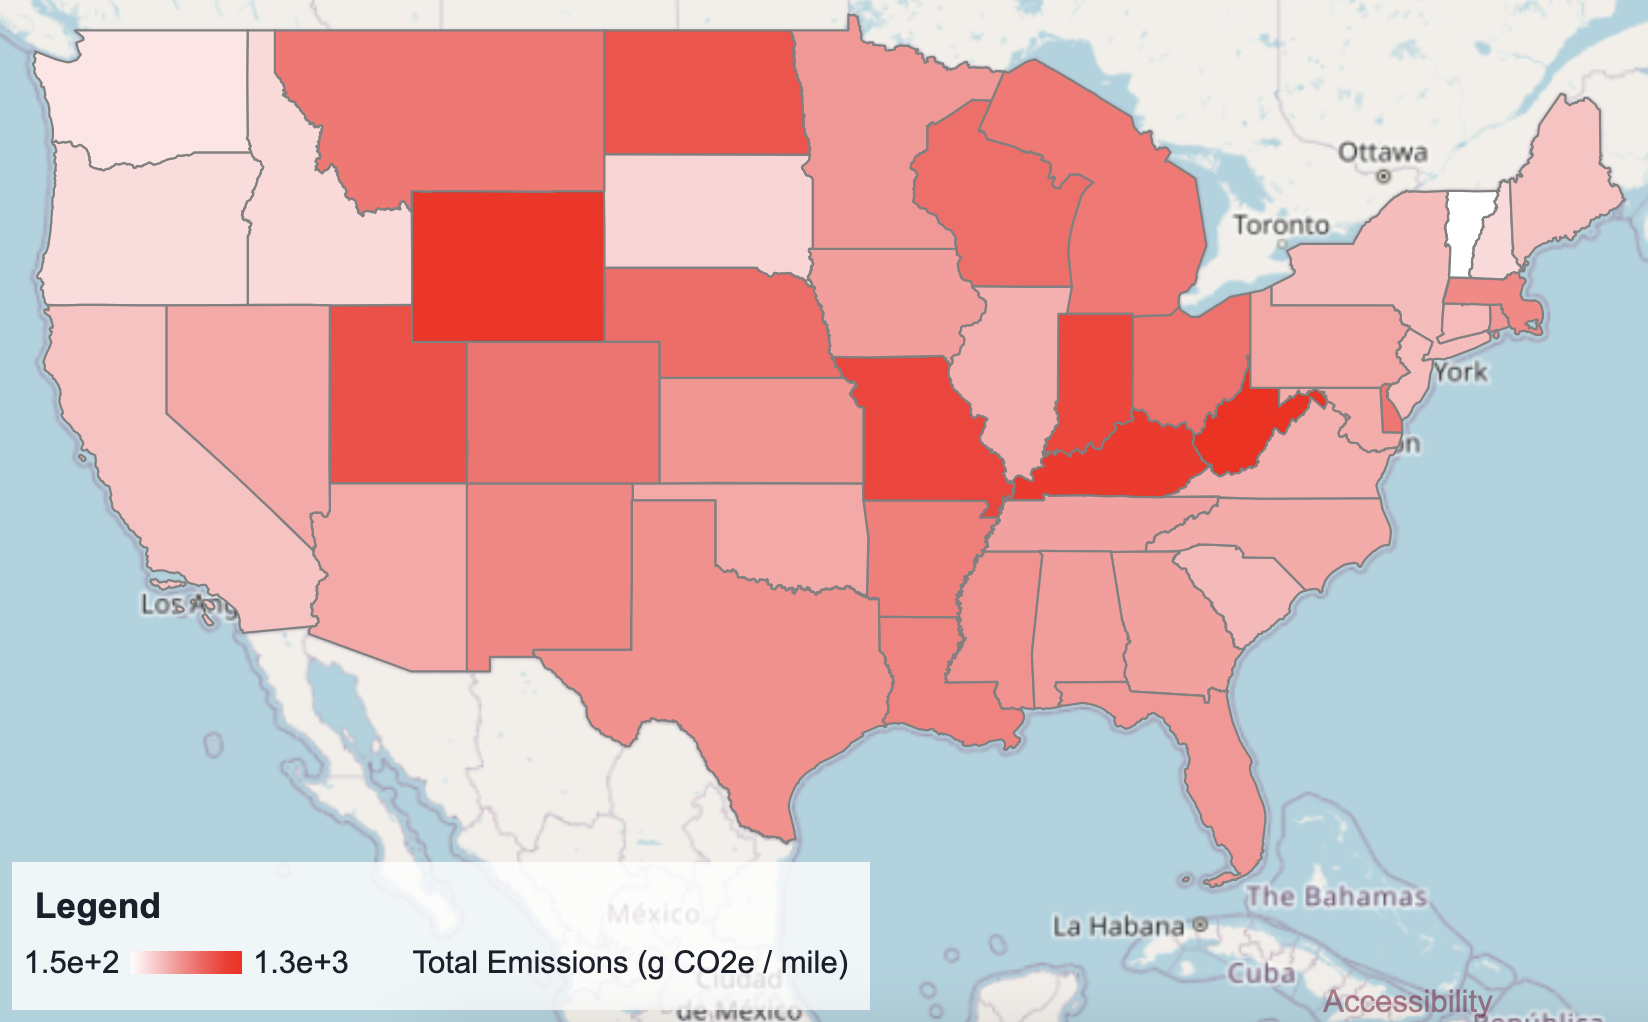
\includegraphics[width=\textwidth]{figures/lifecycle_emissions.png}
        \caption{Well-to-wheel emissions for EV trucking\newline}
        \label{fig:lifecycle_emissions}
    \end{subfigure}
    \hfill
    \begin{subfigure}[b]{0.49\textwidth}
        \centering
        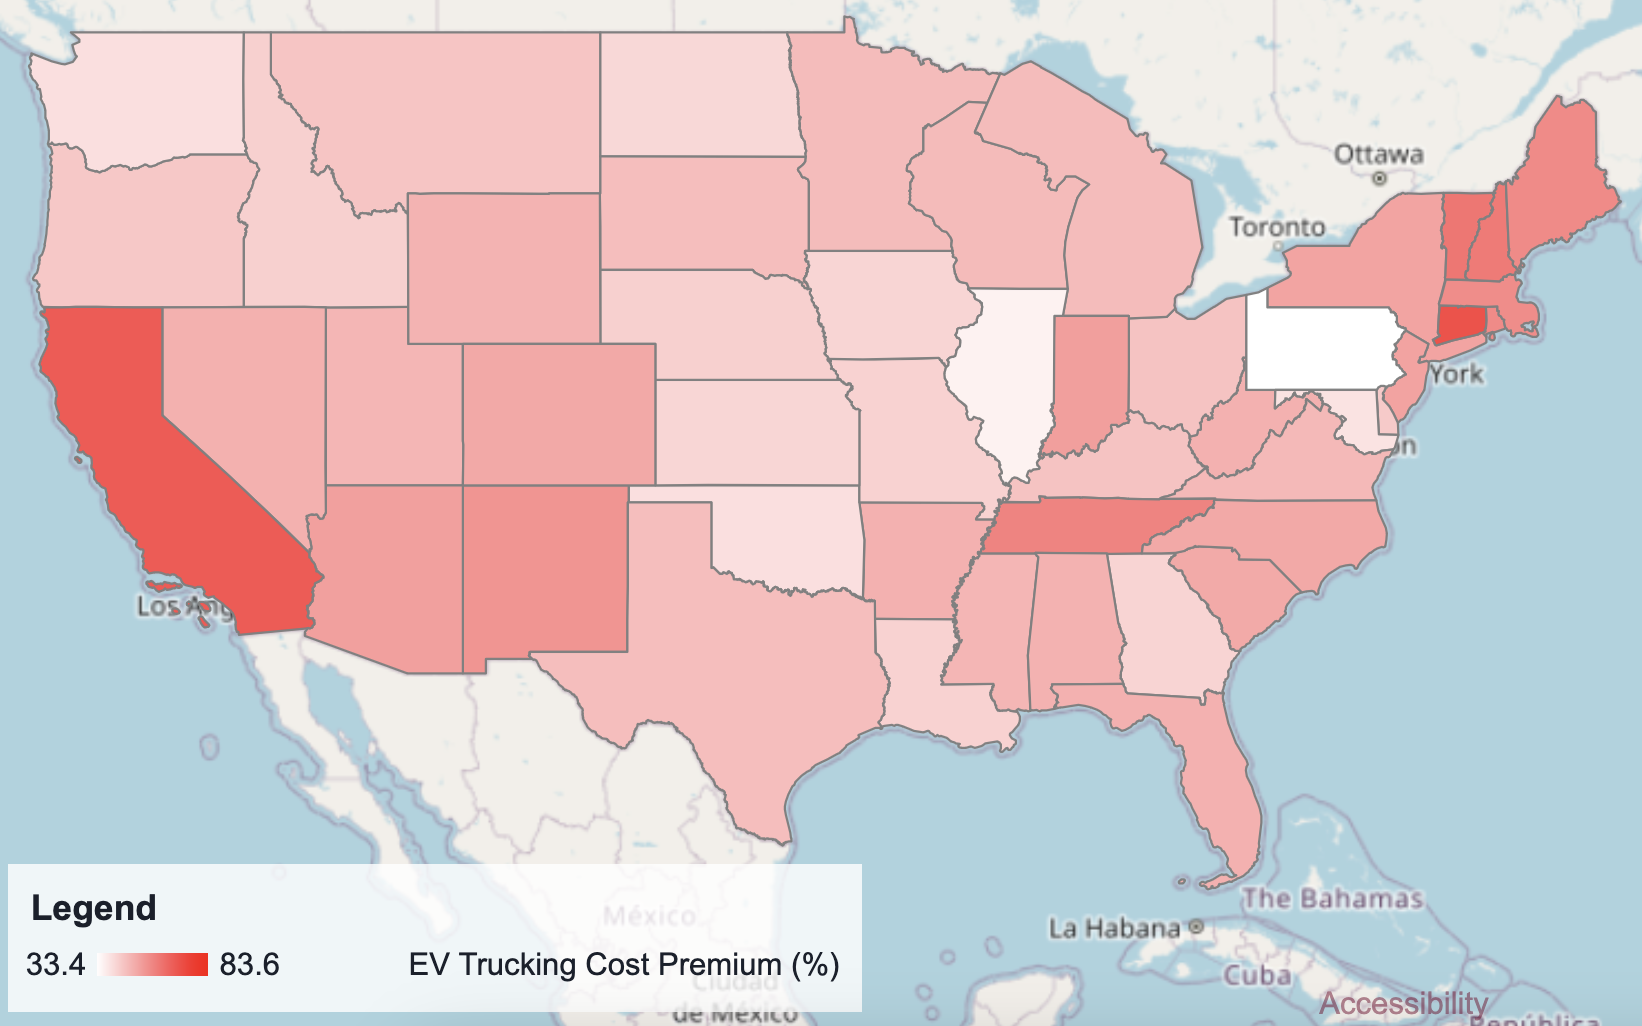
\includegraphics[width=\textwidth]{figures/ev_cost_premium.png}
        \caption{TCO premium for EV trucking, expressed relative to TCO for an equivalent diesel truck}
        \label{fig:ev_cost_premium}
    \end{subfigure}
    \caption{Sample layers used to compare well-to-wheel emissions and total cost of ownership between battery electric and diesel trucking}
    \label{fig:truck_costs_emissions}
\end{figure}

\subsection{State-level Incentives and Regulations}
\label{sec:state_incentives_and_regulations}

The number of incentives and regulations listed on the DOE's Alternative Fuels Data Center \cite{AFDCLaws} to support trucking fleets in transitioning to low-carbon energy carriers are visualized by state. Interactive features presented in Section \ref{sec:interactive_features} allow the user to filter for incentives or regulations separately, or for incentives and regulations targeting specific alternative energy carriers (eg. hydrogen or electricity) or support types (fuel use, infrastructure, or vehicle purchase). As discussed in Section \ref{sec:interactive_features}, the user can also click on specific states to bring up a list of available incentives and regulations matching the specified filters, along with links to more information on the Alternative Fuels Data Center website \cite{AFDCLaws}.

\subsection{Electricity Demand and Capacity}

To help stakeholders compare the grid's ability to support electrified charging demand at the state level, the tool allows users to visualize the total estimated state-level electricity demand associated with charging electric trucks, under a hypothetical scenario in which all present trucking operations along US interstates transition to battery electric. This demand for EV charging can be compared with various quantifiers of the overall state-level capacity and load on the grid to assess its potential impact. 

Figure \ref{fig:ev_charging_demand_load} compares the state-level demand associated with electrified trucking with the total load from all power sources in 2022, indicating that charging demand for a fully electrified US trucking fleet would represent between 2\% and 15\% of the estimated average excess energy capacity available on the grid over the course of a year, depending on the state. 

\begin{figure}[ht]
    \centering
    \begin{subfigure}[b]{0.49\textwidth}
        \centering
        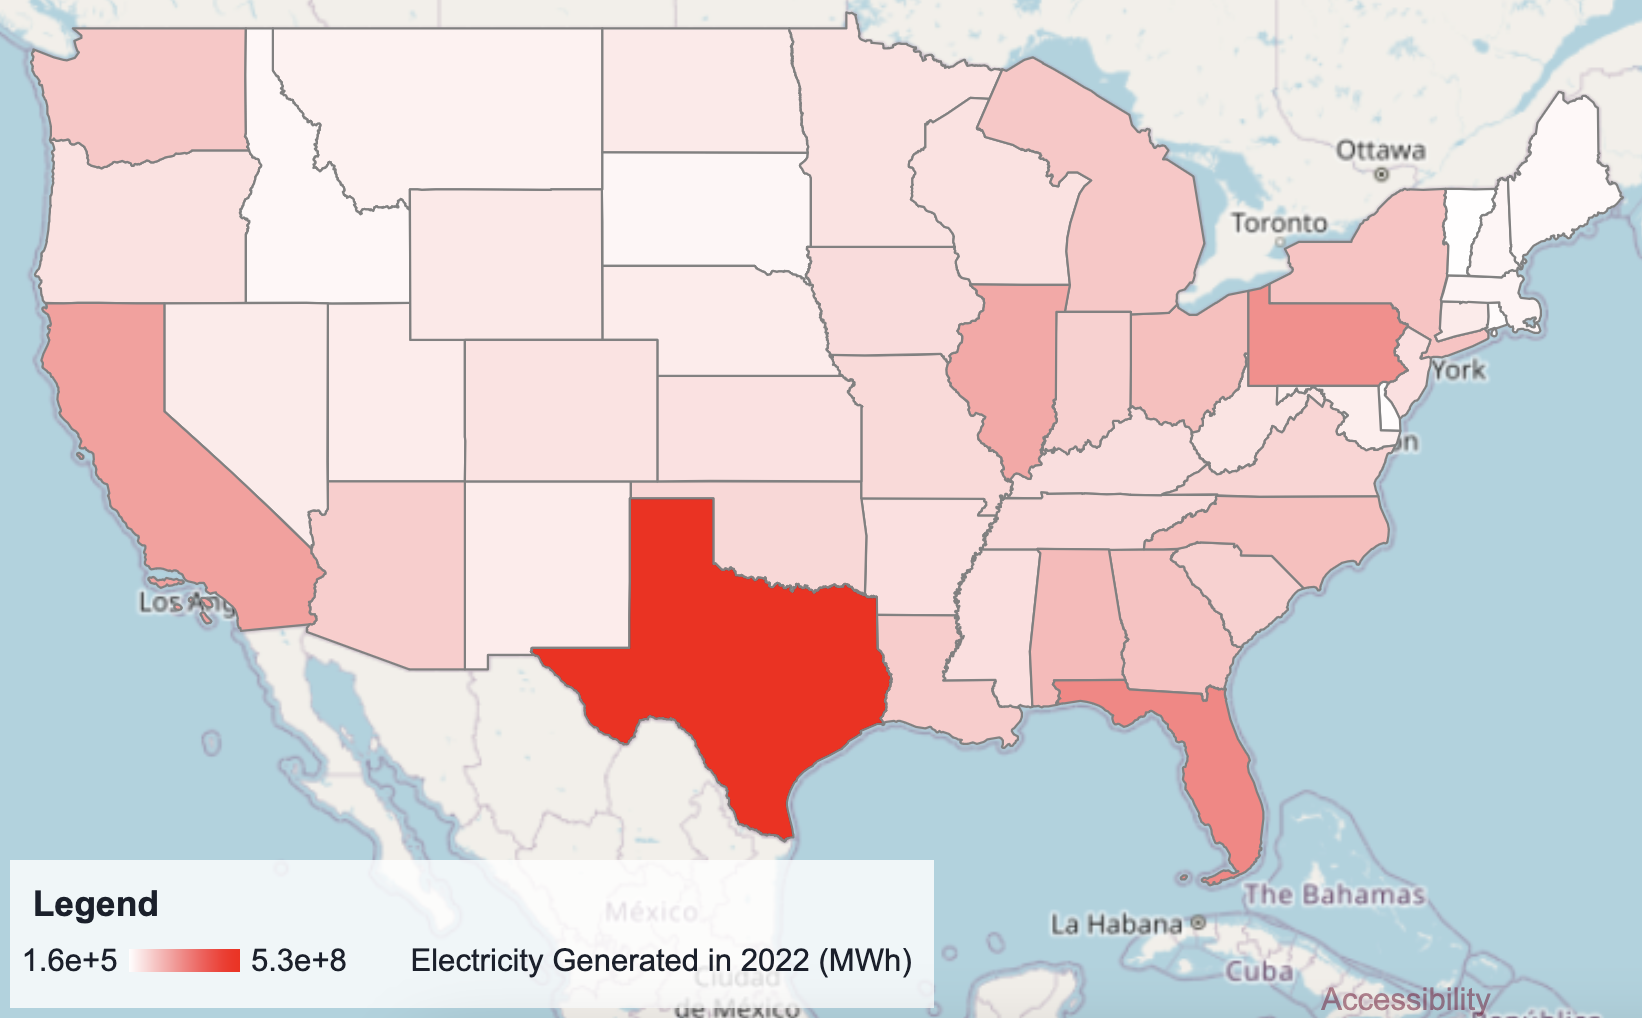
\includegraphics[width=\textwidth]{figures/ev_charging_demand.png}
        \caption{Electricity demand}
        \label{fig:ev_charging_demand}
    \end{subfigure}
    \hfill
    \begin{subfigure}[b]{0.49\textwidth}
        \centering
        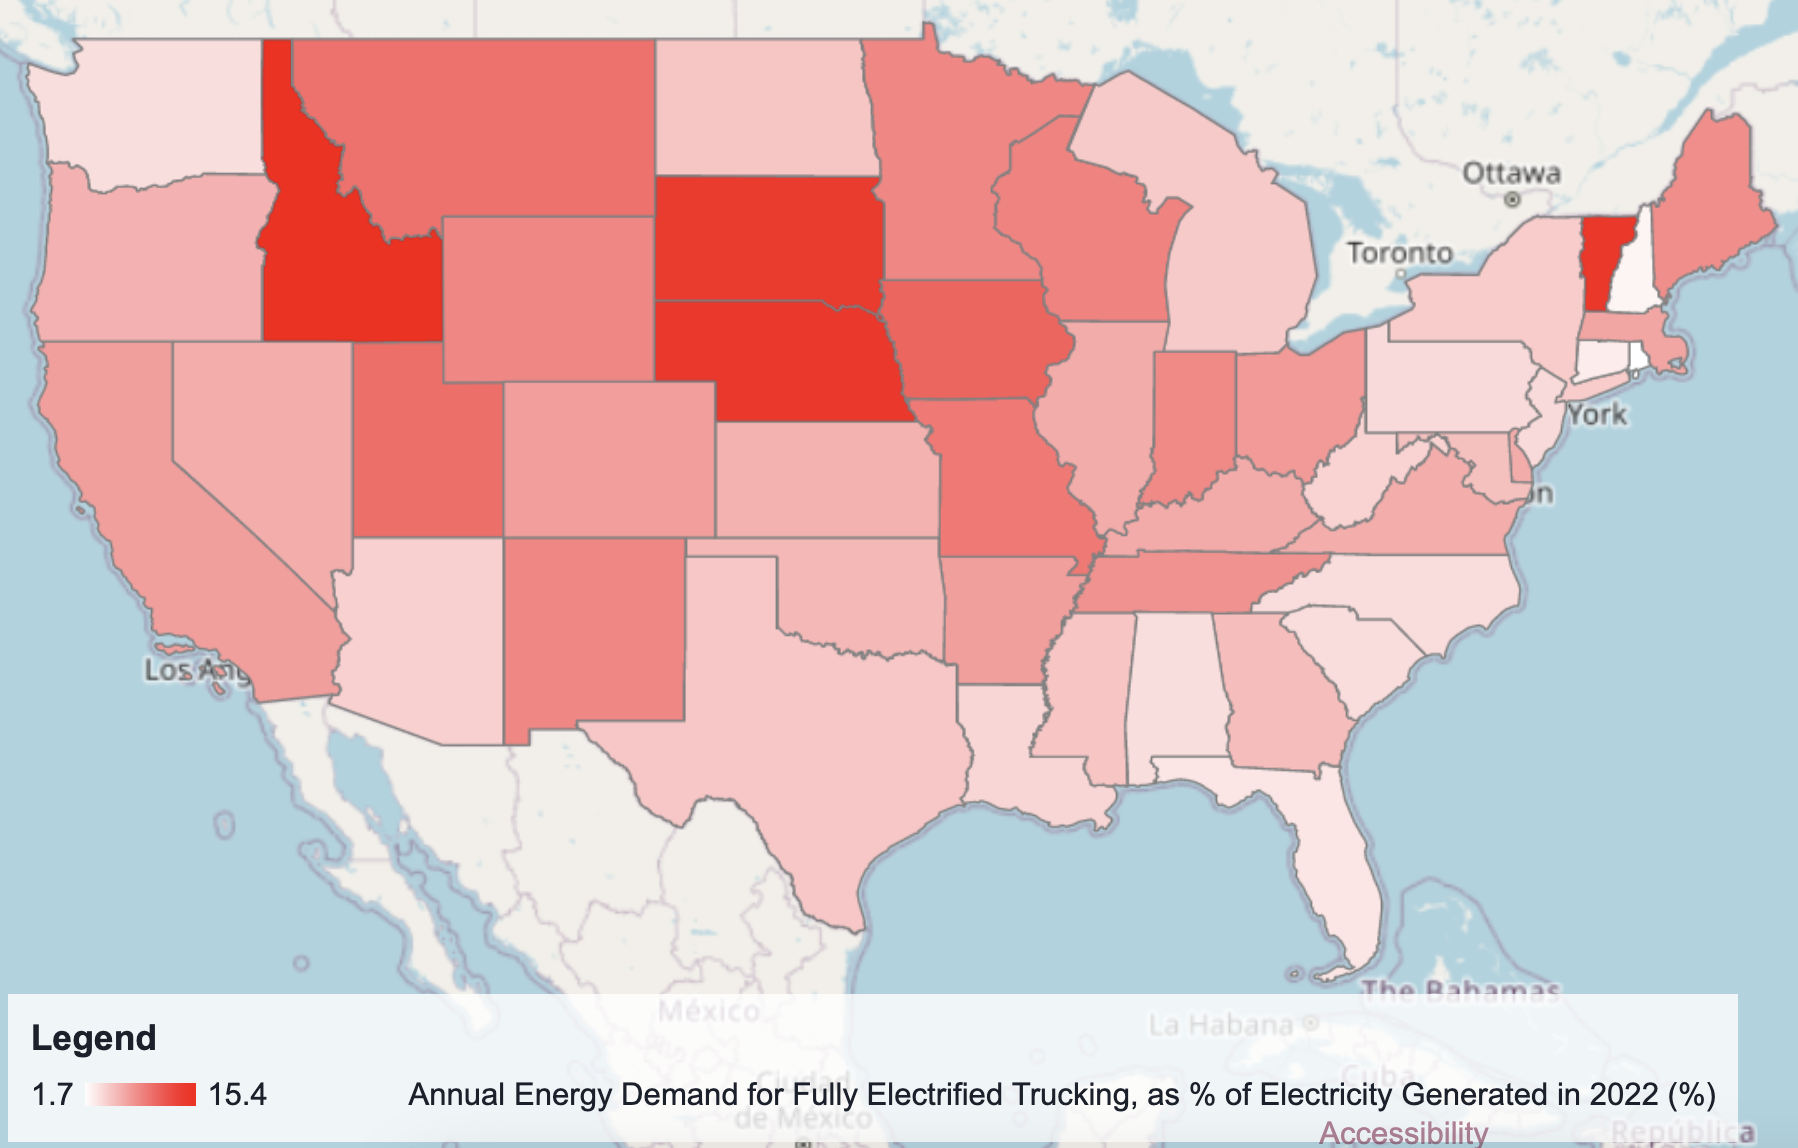
\includegraphics[width=\textwidth]{figures/ev_charging_demand_rel_to_load.png}
        \caption{Relative to annual load}
        \label{fig:ev_charging_demand_rel_to_load}
    \end{subfigure}
    \caption{Left: Annual electricity demand by state for a fully electrified US trucking fleet}
    \label{fig:ev_charging_demand_load}
\end{figure}

The methodology and assumptions used to evaluate these layers are discussed in more detail in Section \ref{sec:demand_capacity}.

\subsection{Pooled Demand for Truck Stop Charging}

The tool also includes a set of point feature accessed through the \text{Truck Stop Charging} checkbox, which are designed to illustrate an exploration presented in Ref. \cite{MacDonell_2024} of potential benefits of pooling charging infrastructure investments among multiple fleets.